% Chapter 4 (Shortened)

\chapter{Results}\label{Chapter4}

%----------------------------------------------------------------------------------------
%	SECTION 1
%----------------------------------------------------------------------------------------

\section{Exploratory Data Analysis}
Following Tier-1 filtering (Chapter~\ref{Chapter3}) and removal of all assessments lacking any cognitive measures, the remaining dataset consisted of 17{,}406 assessments from 7{,}285 patients. The resulting matrix included cognitive variables amounting to 14 variables over six domains. The percentages of missing values are provided in Table~\ref{tab:missing_descriptive}.



Data availability is inconsistent. The missingness levels vary from 0.7\% for Orientation items through to 27.8\% for ATMTA. Therefore, complete-case analysis would lose approximately half of the total clinical sample (46.9\%) and introduce clear selection bias \parencite{rubin1976inference}. Consequently, data imputation was adopted to conserve the entire clinical sample.



From a co-occurrence heatmap (not shown), blocks of variables are identified that are missing simultaneously, suggesting a missing-at-random mechanism \parencite{rubin1976inference,little2019statistical}. Dependency among missing values thus supports the application of conditional imputation rather than naive substitution. Within-domain correlation coefficients are generally high, whereas cross-domain relationships appear less prominent, suggesting common variance due to general cognitive ability \parencite{lezak2012neuropsychological}. Subsequent clustering results illustrate this common variance dimension explicitly.

\begin{table}[ht]
\caption{Missingness summary for the 14 eligible neuropsychological variables after Tier~1 filtering. The final row reports the number of complete cases (rows with no missing values across all 14 variables).}
\label{tab:missing_descriptive}
\centering
\small
\begin{tabular}{l l r r r}
\toprule
\textbf{Variable} & \textbf{Domain} & \textbf{$N$ Observed} & \textbf{$N$ Missing} & \textbf{Missing \%} \\
\midrule
\texttt{OTEMPS}          & Orientation        & 17{,}286 &   120 &  0.7 \\
\texttt{OPERSONA}        & Orientation        & 17{,}284 &   122 &  0.7 \\
\texttt{OESPAI}          & Orientation        & 17{,}282 &   124 &  0.7 \\
\texttt{ASPAN}           & Attention          & 15{,}611 & 1{,}795 & 10.3 \\
\texttt{MRAVLT075}       & Memory             & 15{,}523 & 1{,}883 & 10.8 \\
\texttt{MDIGITS}         & Memory             & 15{,}373 & 2{,}033 & 11.7 \\
\texttt{FEPMR}           & Executive Function & 14{,}682 & 2{,}724 & 15.6 \\
\texttt{LCOMPRENSIOTB}   & Language           & 14{,}686 & 2{,}720 & 15.6 \\
\texttt{LDENOMINACIOTB}  & Language           & 14{,}677 & 2{,}729 & 15.7 \\
\texttt{LREPETICIOTB}    & Language           & 14{,}634 & 2{,}772 & 15.9 \\
\texttt{MRAVLT015}       & Memory             & 14{,}281 & 3{,}125 & 18.0 \\
\texttt{MRAVLT015R}      & Memory             & 14{,}199 & 3{,}207 & 18.4 \\
\texttt{VPIMATGES}       & Visuoperception    & 12{,}992 & 4{,}414 & 25.4 \\
\texttt{ATMTA}           & Attention          & 12{,}575 & 4{,}831 & 27.8 \\
\midrule
\multicolumn{3}{l}{\textbf{Complete cases (all 14 variables observed)}} & \multicolumn{2}{r}{\textbf{9{,}245 (53.1\%)}} \\
\bottomrule
\end{tabular}
\end{table}

In Figure~\ref{fig:missingness_barplot}, missingness levels for each cognitive variable are displayed in descending order. Highly specialized assessments consistently demonstrate higher levels of missingness than routine screening measures \parencite{lezak2012neuropsychological}.

\begin{center}
\centering
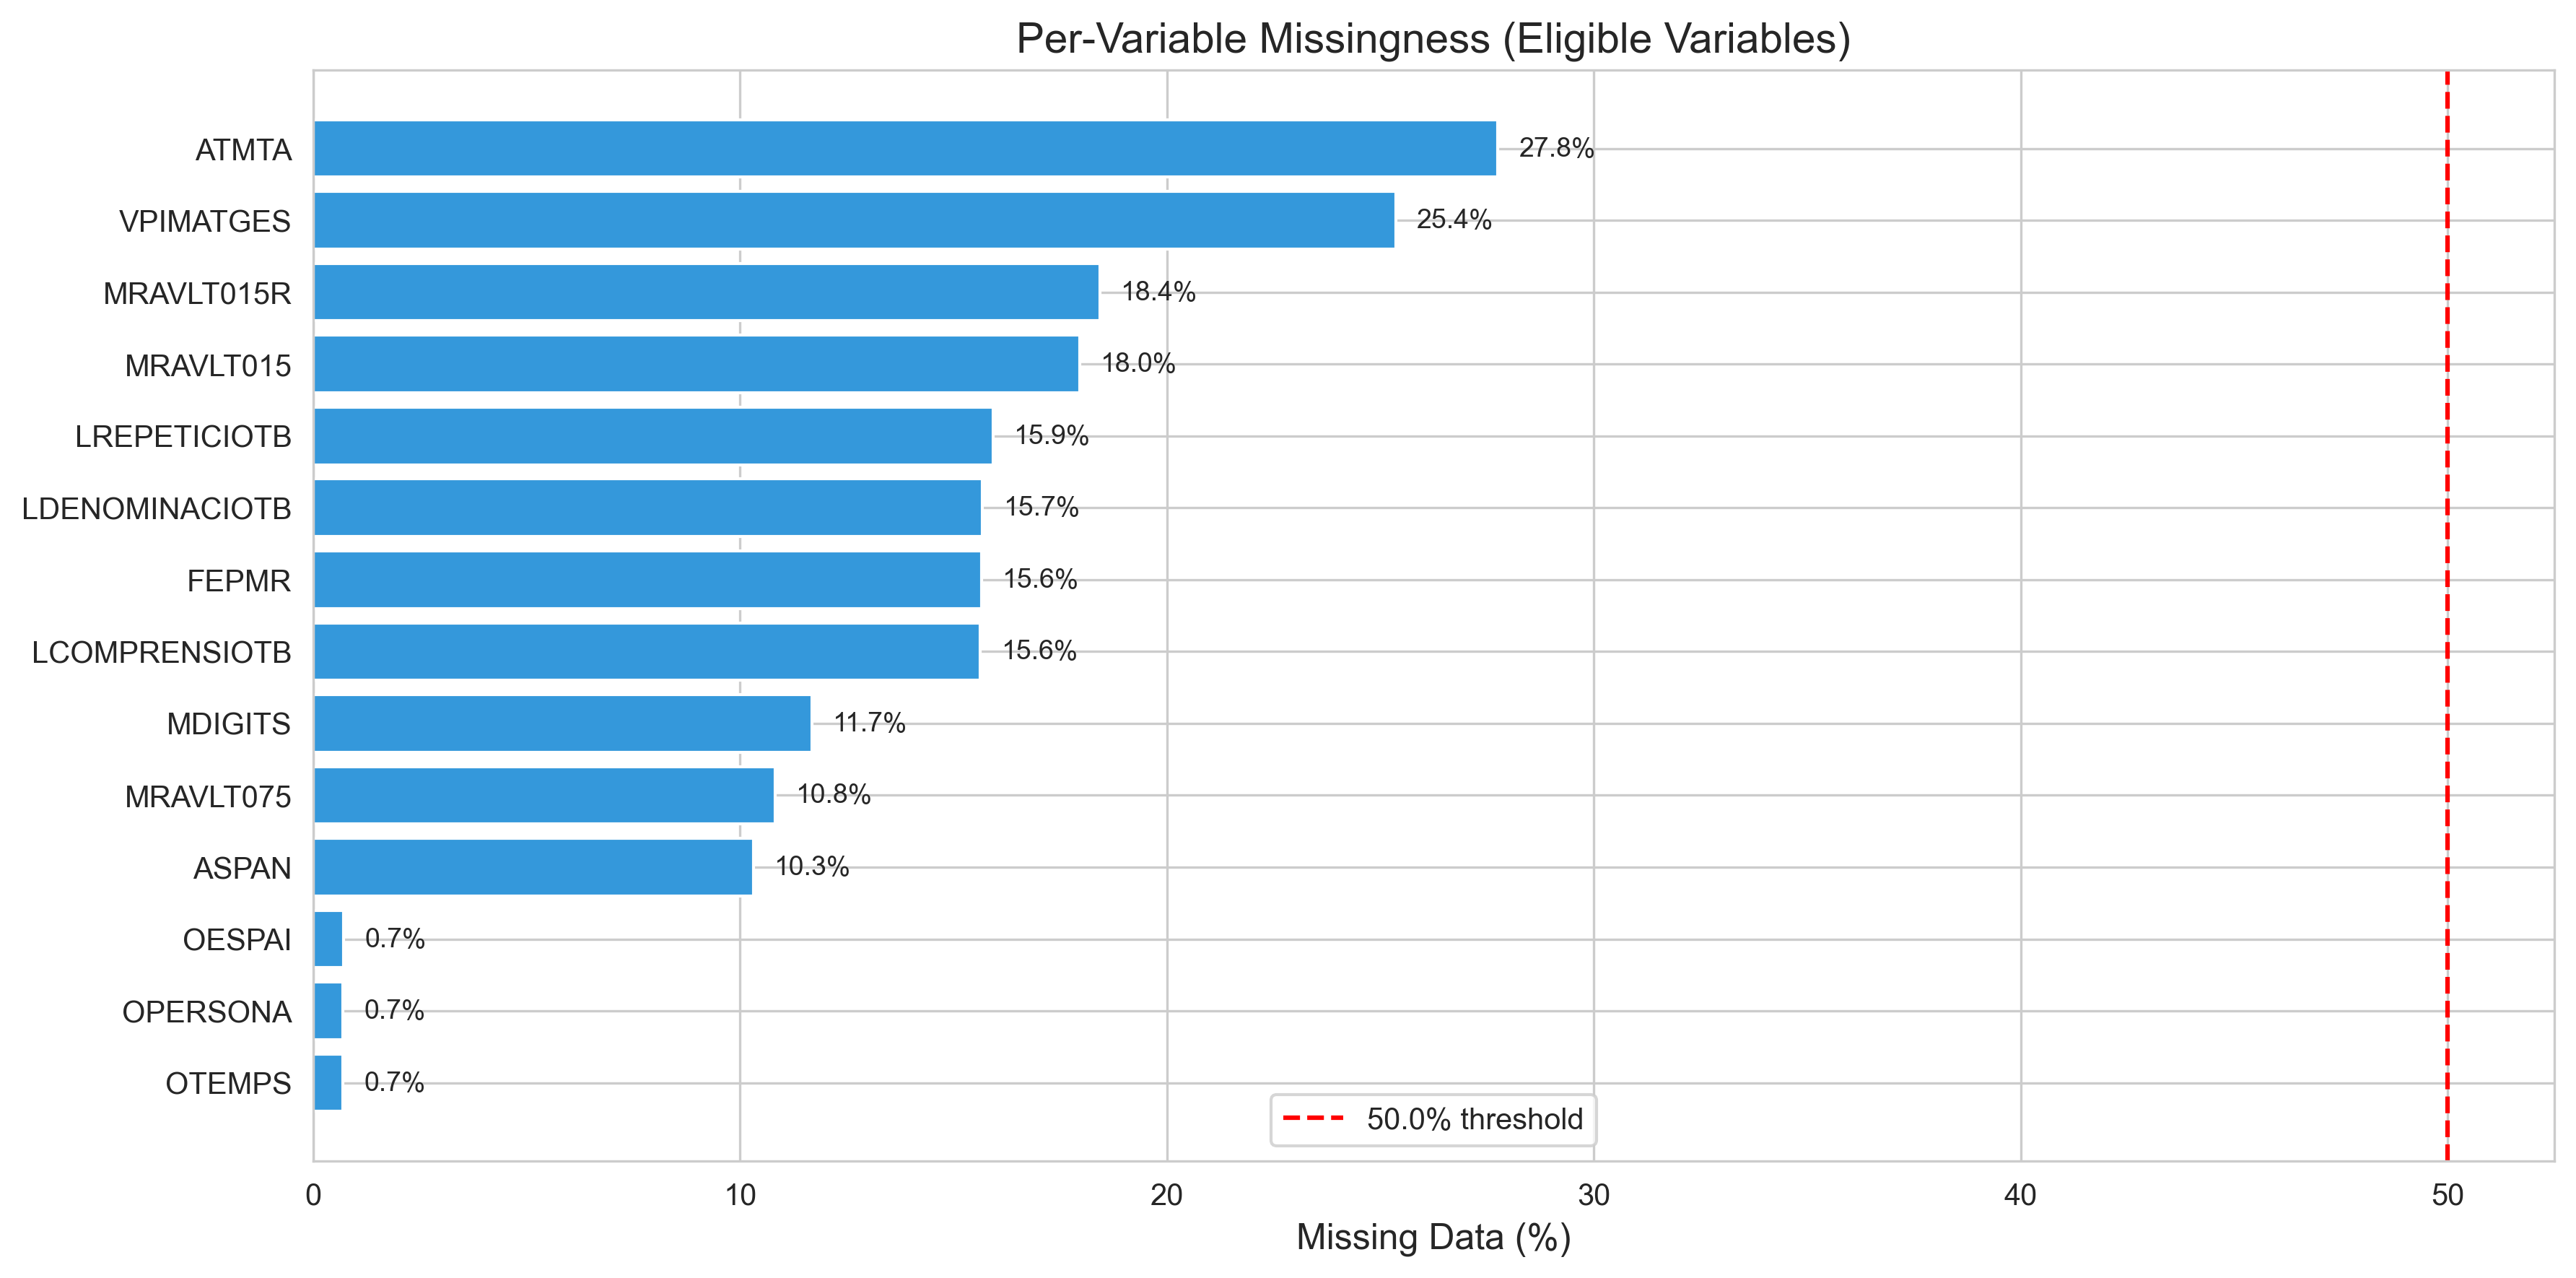
\includegraphics[width=0.9\textwidth]{Figures/missingness_barplot.png}
\captionof{figure}[Missingness rates by variable]{Missingness bar plot for all cognitive variables, ordered by missingness rates. Missingness rates were higher among the specialised assessments compared to the routine screening assessments.}
\label{fig:missingness_barplot}
\end{center}

\section{Imputation Results}
Prior to conducting clustering evaluations on their respective datasets, I tested all ten imputation techniques represented in Figure~\ref{fig:imputation_comparison} and Figure~\ref{fig:imputation_comparison_b}. Due to compression of variance \parencite{rubin1987multiple}, Mean Imputation behaves differently from all other methods. All nine remaining methods maintain closer adherence to marginal distributions. Discrete structure retention is greater among donor-based methods like KNN and PMM than among model-based approaches including MICE, MissForest and EM that produce smoothed continuous reconstructions.

\begin{center}
\centering
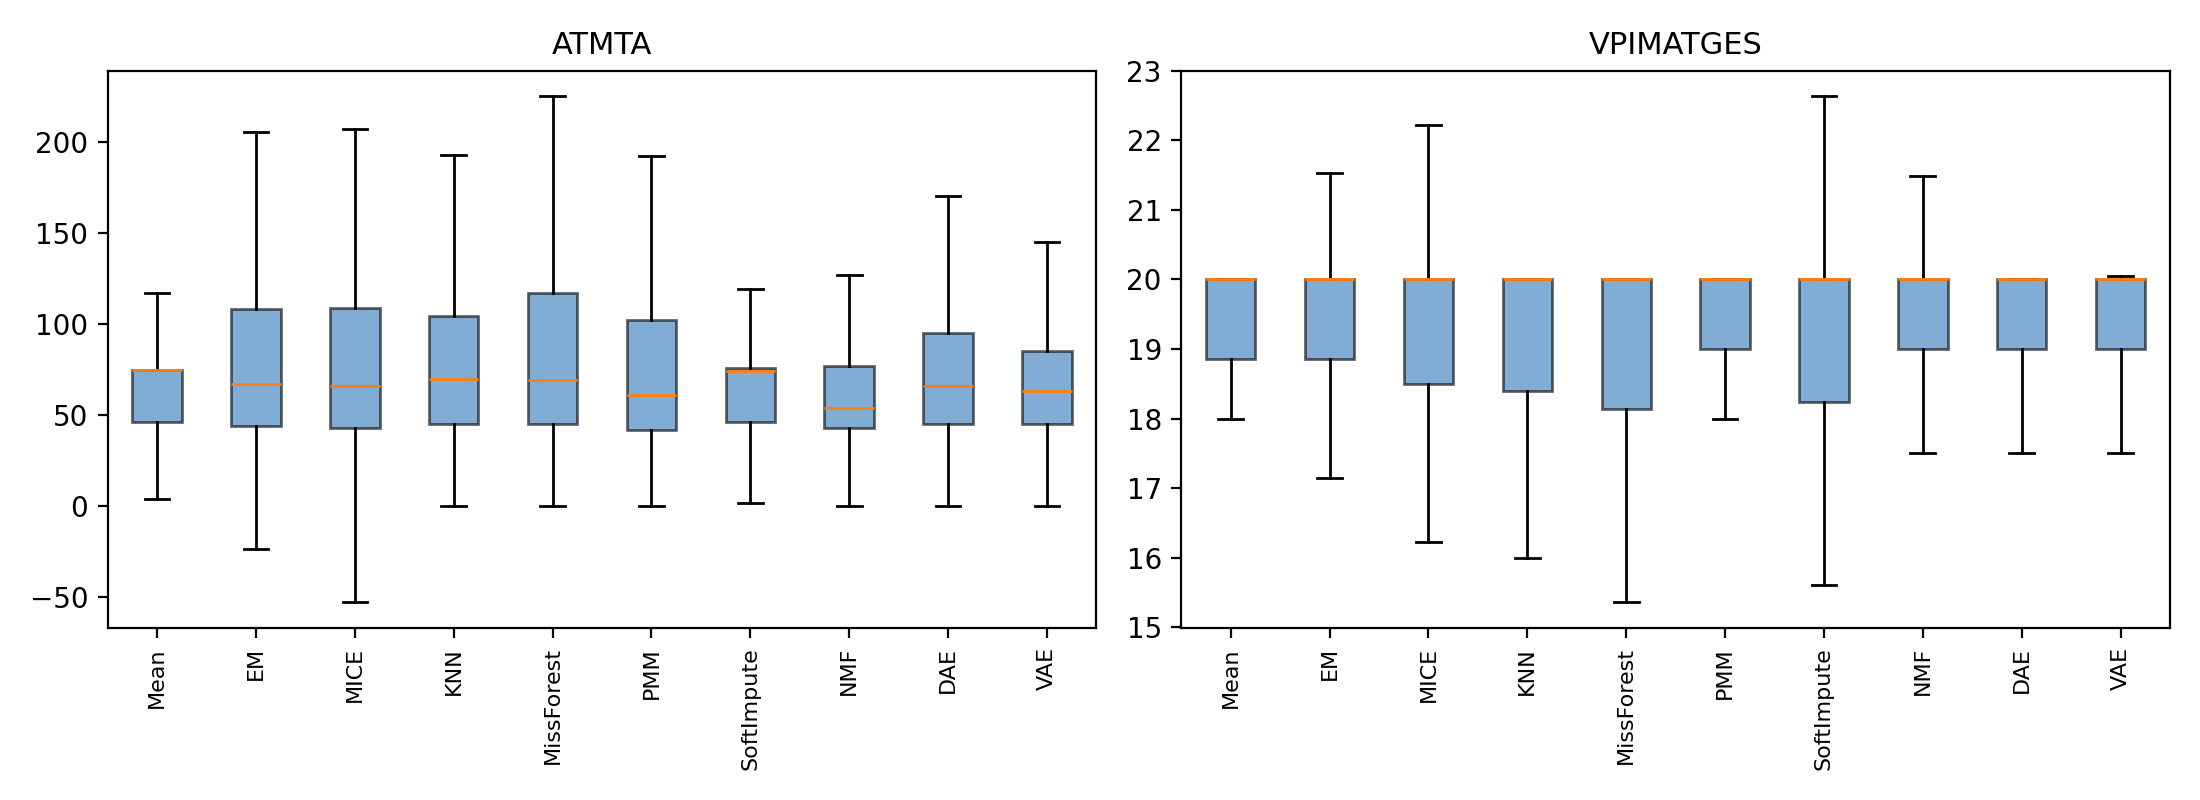
\includegraphics[width=0.95\textwidth]{Figures/imputation_comparison_boxplots_a.png}
\captionof{figure}[Imputation comparison (ATMTA, VPIMATGES)]{Comparison of distributions for each of the 10 different imputation methods for ATMTA and VPIMATGES. Mean imputation reduces variance whereas model-based methods maintain the distributional characteristics of the original data.}
\label{fig:imputation_comparison}
\end{center}

\begin{center}
\centering
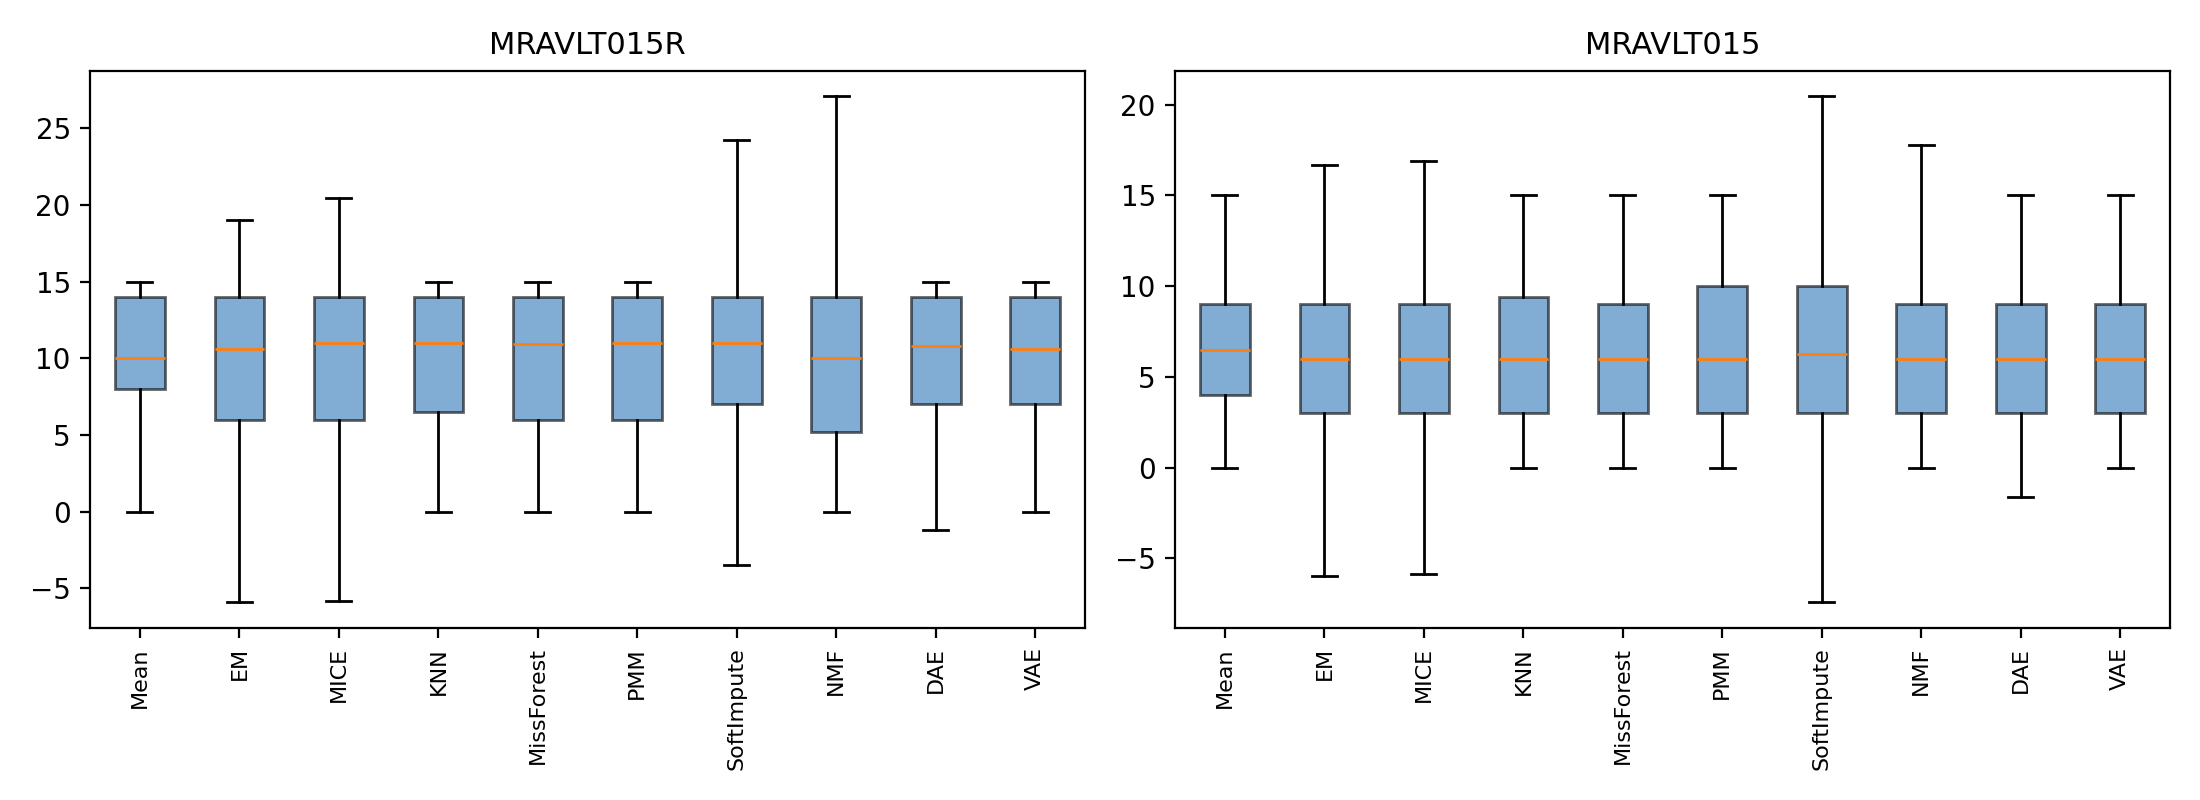
\includegraphics[width=0.95\textwidth]{Figures/imputation_comparison_boxplots_b.png}
\captionof{figure}[Imputation comparison (MRAVLT015R, MRAVLT015)]{Comparison of distributions for MRAVLT015R and MRAVLT015. Deep learning models (DAE, VAE) closely approximate model-based methods.}
\label{fig:imputation_comparison_b}
\end{center}

\section{Baseline and Primary Clustering}
I first fitted K-means and Gaussian mixture baselines across \(k=2\) through \(k=6\). Neither produced a clear discrete optimum: the K-means elbow lacked a pronounced break, and silhouette was highest at \(k=2\) but declined as additional groups were introduced. These baselines motivated examination of density structure; they were not treated as evidence that natural cognitive classes existed.

I selected HDBSCAN because it can recover irregularly shaped dense regions, represent low-density observations as noise, and examine cluster persistence across a hierarchy without requiring a fixed value of \(k\). This combination was appropriate for routine clinical data in which boundary cases may not fit cleanly into a group. UMAP was repeated across ten random seeds per parameter configuration, and HDBSCAN was evaluated over the 120-configuration grid described in Chapter~\ref{Chapter3}. The comparison of t-SNE and UMAP in Figure~\ref{fig:tsne_umap} is descriptive: it illustrates how the selected assignments appear under two projections, but it is not an independent test of cluster existence or discreteness.

\begin{sloppypar}
For the UMAP+HDBSCAN combination, the hyperparameters I settled on were: \texttt{n\_components}$=8$, \texttt{n\_neighbors}$=15$, and \texttt{min\_dist}$=0.0$ for UMAP (to allow for tight packing in the embedding space \parencite{mcinnes2018umap}); and for HDBSCAN, \texttt{min\_cluster\_size}$=1000$ and \texttt{min\_samples}$=50$ with \texttt{cluster\_selection\_method}$=\text{eom}$ and \texttt{epsilon}$=0.0$. I chose a large cluster size to ensure that only substantive groupings are retained.
\end{sloppypar}

\begin{center}
\centering
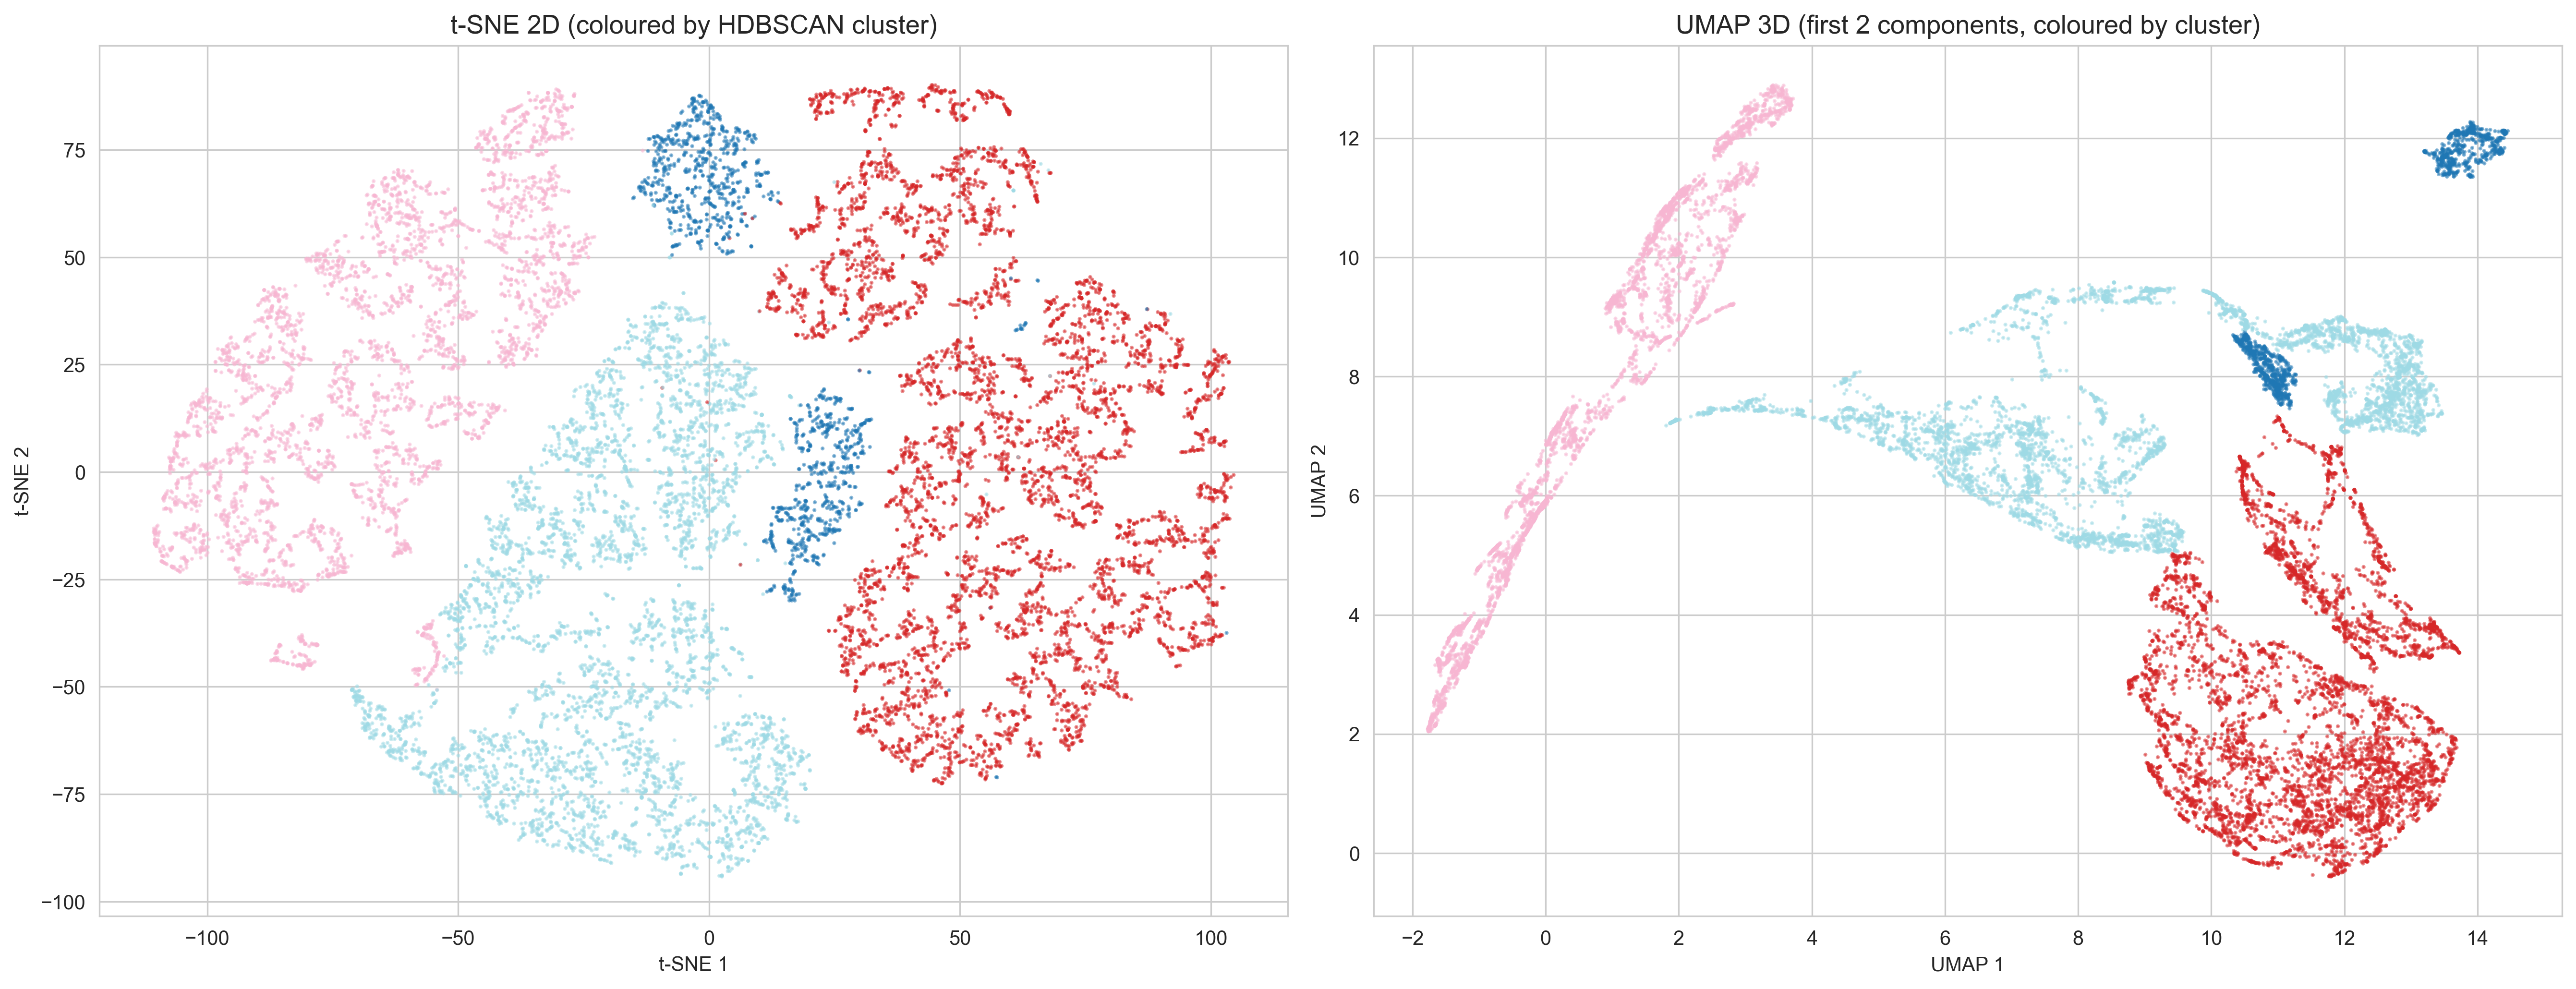
\includegraphics[width=0.9\textwidth]{Figures/tsne_umap_clusters.png}
\captionof{figure}[t-SNE and UMAP cluster projections]{Two-dimensional representations of the data using t-SNE (left) and UMAP (right), with HDBSCAN cluster assignments coloured. UMAP reveals clearer separation of cluster areas.}
\label{fig:tsne_umap}
\end{center}

\section{Cognitive Profiles of the Clusters}\label{sec:cluster_profiles}
Below are the radar plots showing mean cognitive domain score per tier, expressed as a z-score from the cohort mean. The three polygons are roughly concentric (every domain moves together), so the tiers differ in overall level rather than in profile shape.



Additionally, I created a random forest surrogate that attempts to recover the tier labels from the domain scores. The Gini importance for each domain shows which domains contribute most strongly to distinguishing among tiers. There is considerable inter-correlation between the domain scores (because they are all based on cognitive performance), so interpreting this figure requires caution: although Attention appears to have low Gini Importance relative to Working Memory and Processing Speed, for example, this may simply reflect a high degree of correlation between Attention and Working Memory rather than anything about attention being clinically unimportant.

\begin{center}
\centering
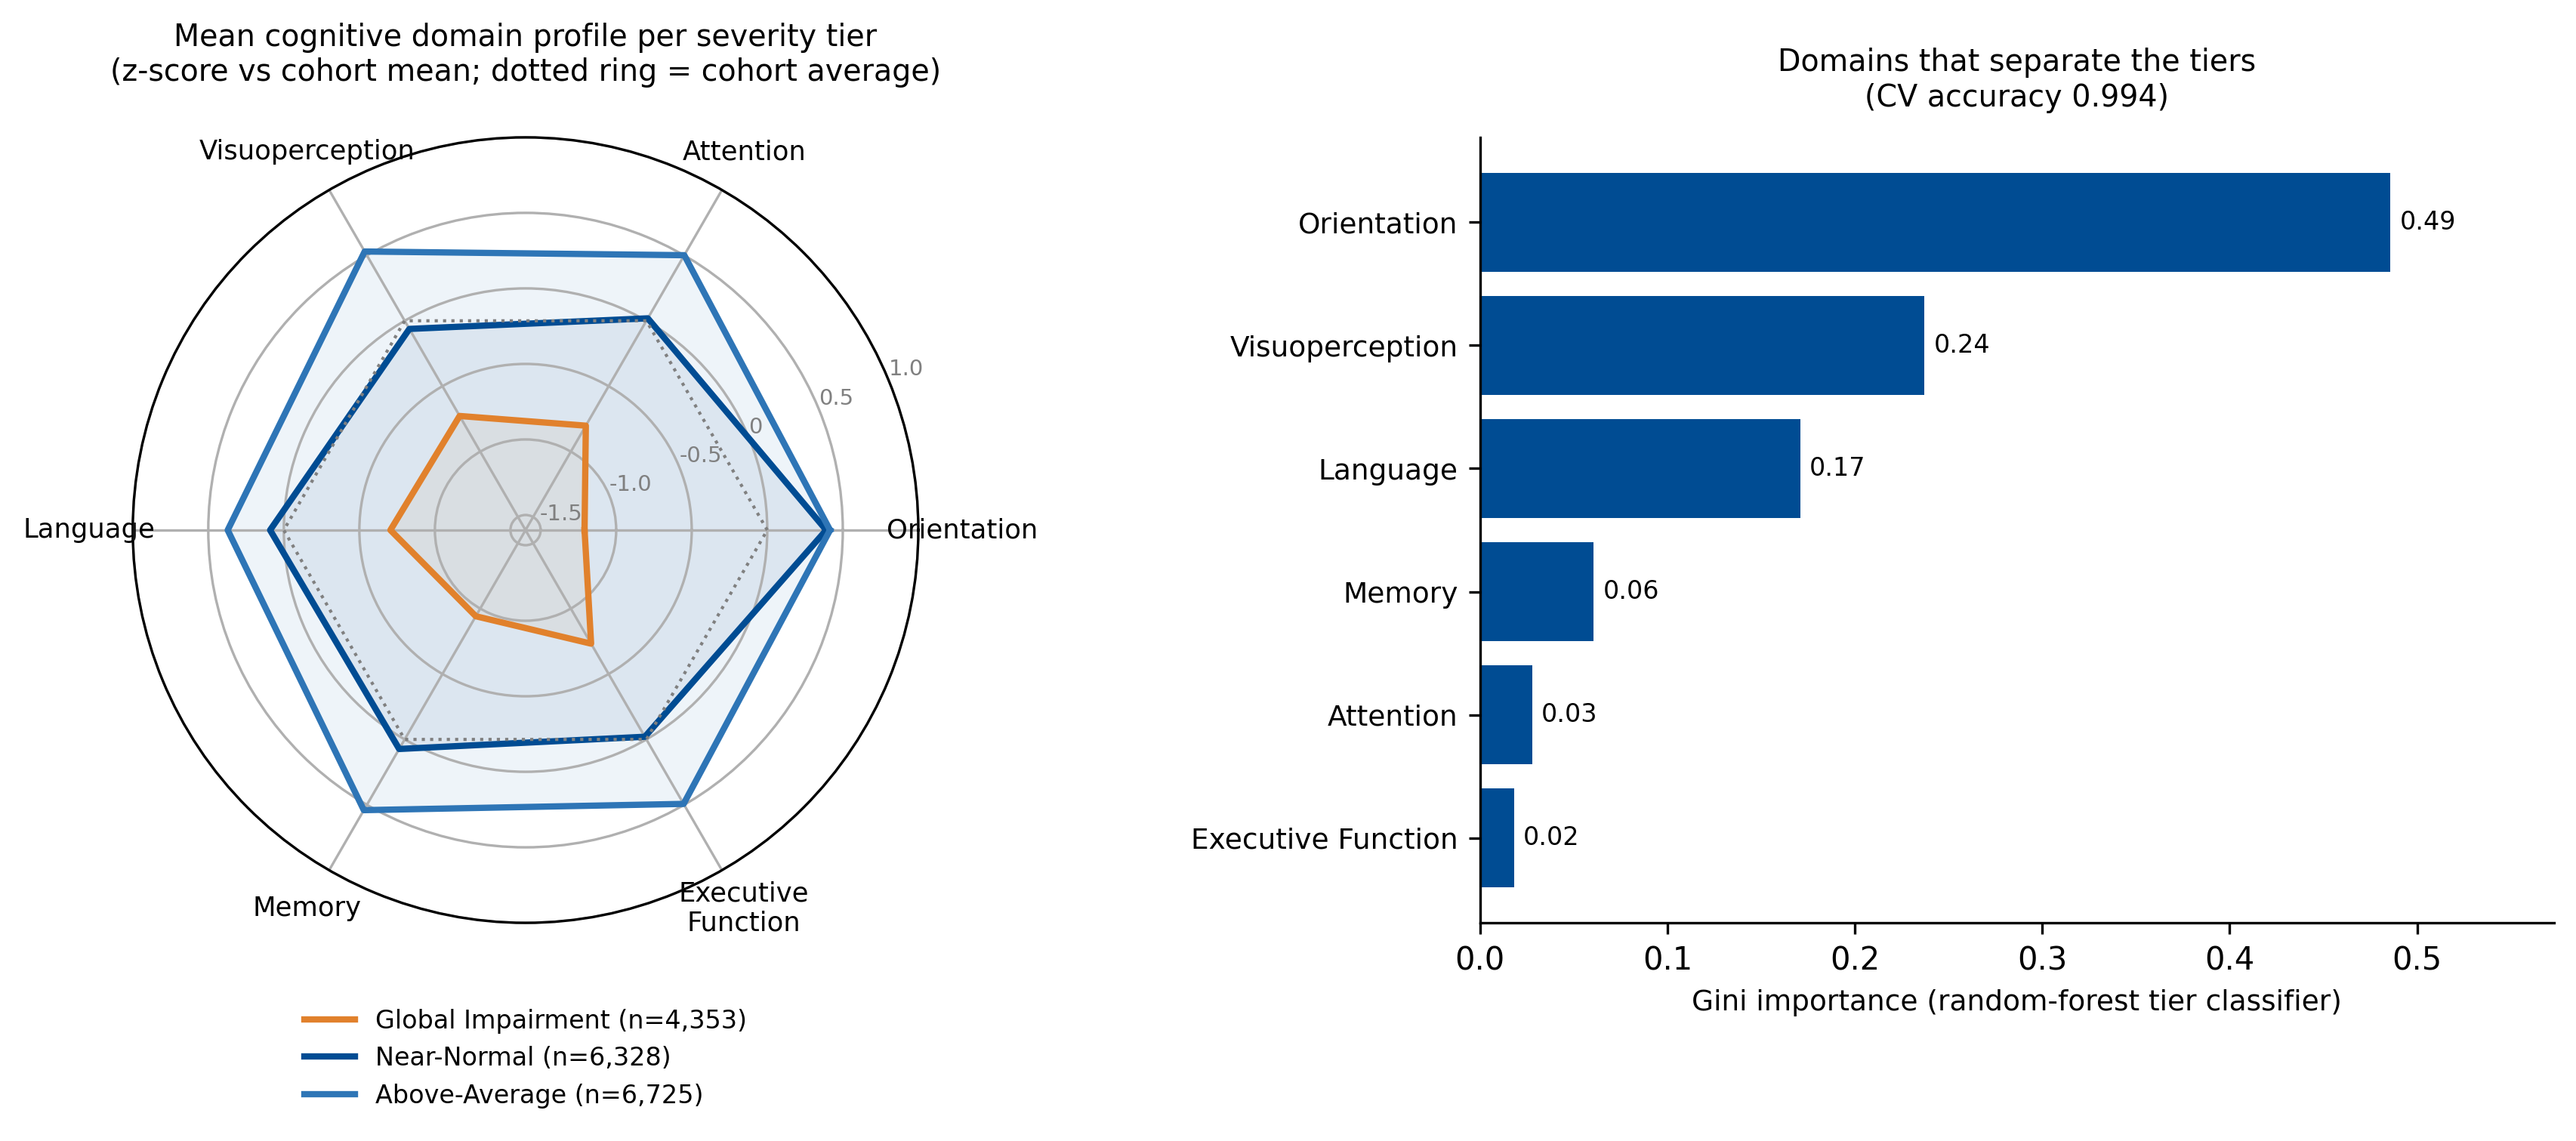
\includegraphics[width=\textwidth]{Figures/cognitive_radar_profiles.png}
\captionof{figure}[Cognitive domain severity profiles]{Left: Mean score for each cognitive domain in each tier, expressed as a z-score from the cohort mean (the dotted ring indicates the cohort average). The three polygons are approximately circular because each domain moves collectively; therefore, the tiers differ in terms of global levels rather than shapes. Right: Gini importance from a random forest surrogate that recovers tier labels from domain scores (accuracy = 0.994). Since these labels are derived from those same scores, this panel describes the decision boundaries of the partitions instead of providing independent importance measurements, and the ordering depends on inter-domain correlation (see Section~\ref{sec:feature_importance}). It should not be interpreted as suggesting that attention has no clinical significance.}
\label{fig:radar_profiles}
\end{center}

\section{Hypothesis 1: Stability and Discreteness}\label{sec:h1_results}
Hypothesis 1 contained two related claims: that reproducible groupings would be recovered and that those groupings would represent discrete cognitive phenotypes. I evaluated stability using 50 bootstrap resamples for each imputation method. HDBSCAN was refitted to each resampled UMAP embedding, and I recorded silhouette, pre-KNN noise proportion, and Hennig core-Jaccard matching. Figure~\ref{fig:h1_bootstrap} shows the bootstrap distributions, while Table~\ref{tab:h1_per_method} reports the exact per-method summaries.

\begin{center}
\centering
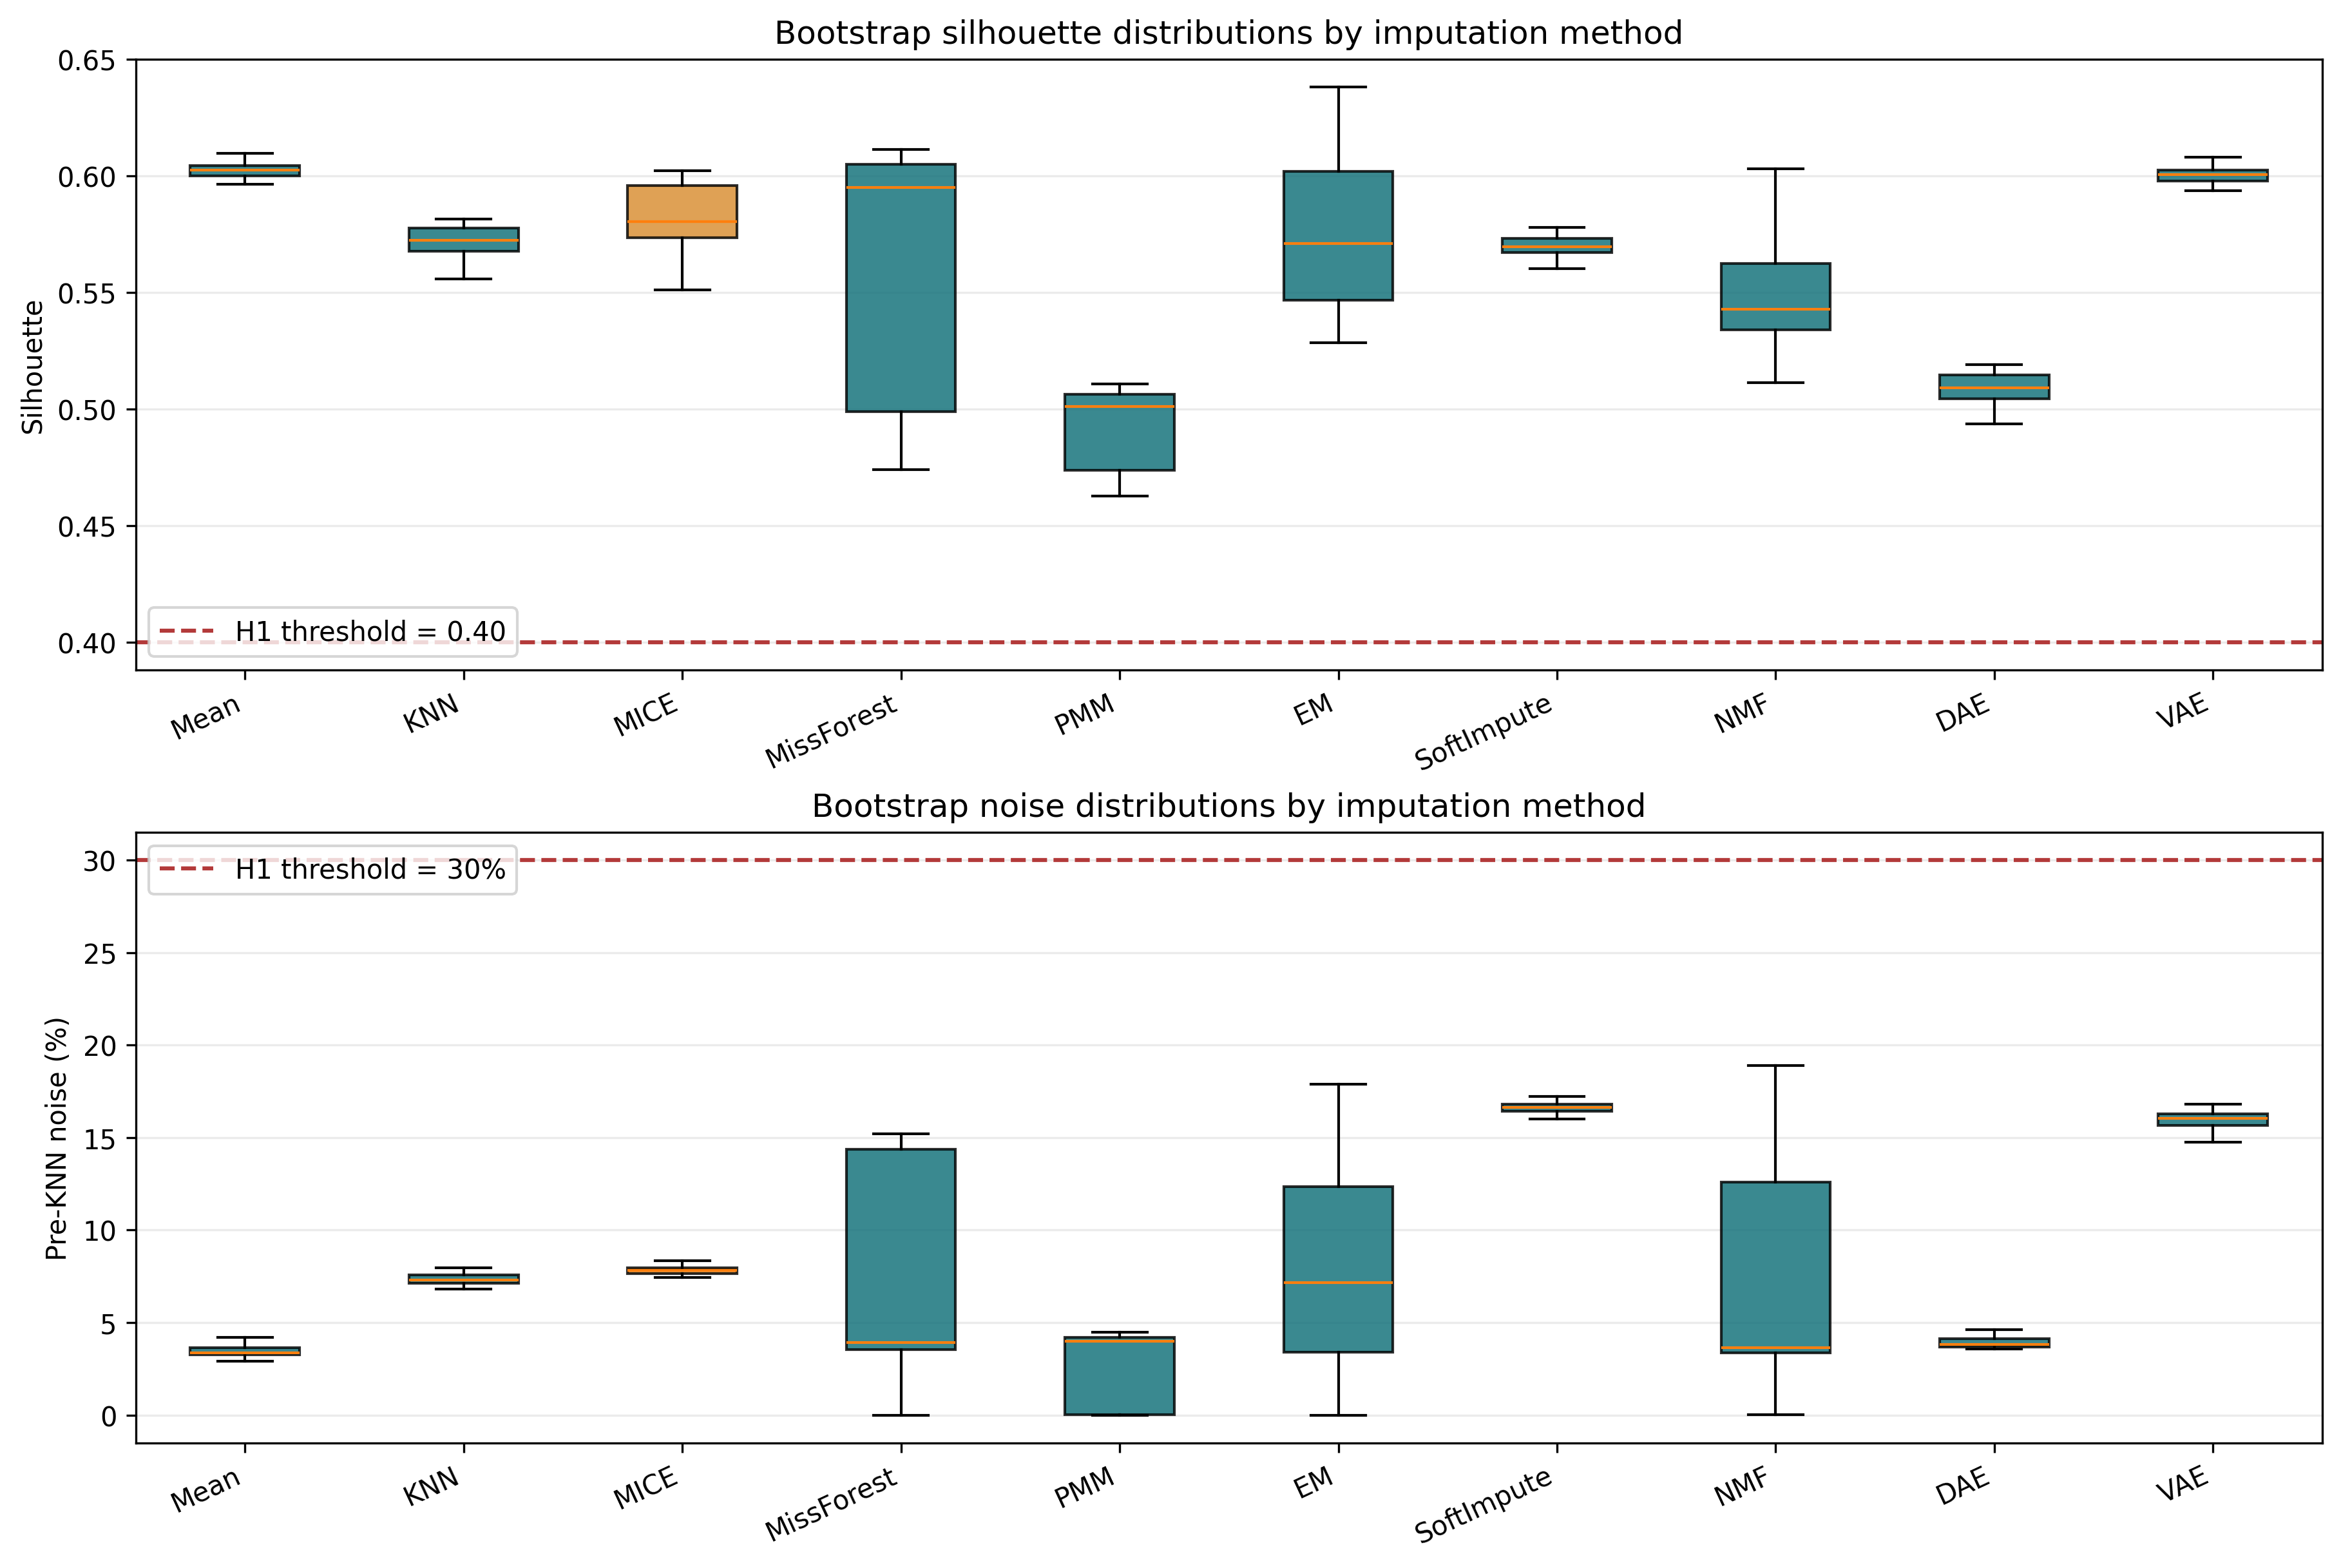
\includegraphics[width=0.92\textwidth]{Figures/h1_bootstrap_distributions.png}
\captionof{figure}[H1 bootstrap stability by imputation method]{Bootstrap distributions of silhouette (top) and pre-KNN HDBSCAN noise proportion (bottom) across 50 assessment-level resamples for each imputation method. Dashed lines mark the pre-specified H1 thresholds. All ten methods met the silhouette and noise criteria, although these values describe stability in the selected UMAP embedding and do not account for repeated assessments within patients.}
\label{fig:h1_bootstrap}
\end{center}

\begin{center}
\small
\captionof{table}[Per-method H1 stability results]{Exact per-method H1 results. Silhouette and noise are bootstrap medians before KNN reassignment. Overall Jaccard is the mean matched-cluster value; the final column gives the range across clusters within each method.}
\label{tab:h1_per_method}
\begin{tabular}{lrrrrr}
\toprule
\textbf{Method} & \textbf{$k$} & \textbf{Silhouette} & \textbf{Noise \%} & \textbf{Jaccard} & \textbf{Cluster range} \\
\midrule
Mean       & 4 & 0.602 &  3.4 & 0.630 & 0.627--0.633 \\
KNN        & 4 & 0.572 &  7.3 & 0.600 & 0.543--0.632 \\
MICE       & 3 & 0.581 &  7.8 & 0.573 & 0.467--0.630 \\
MissForest & 3 & 0.595 &  3.9 & 0.570 & 0.536--0.631 \\
PMM        & 4 & 0.501 &  4.0 & 0.615 & 0.580--0.631 \\
EM         & 4 & 0.571 &  7.1 & 0.509 & 0.383--0.630 \\
SoftImpute & 4 & 0.570 & 16.6 & 0.610 & 0.586--0.631 \\
NMF        & 3 & 0.543 &  3.6 & 0.584 & 0.557--0.631 \\
DAE        & 5 & 0.509 &  3.8 & 0.566 & 0.490--0.630 \\
VAE        & 4 & 0.601 & 16.0 & 0.600 & 0.574--0.631 \\
\bottomrule
\end{tabular}
\end{center}

All ten methods passed the pre-specified silhouette and noise thresholds. However, strict per-cluster reproducibility was weaker: overall core Jaccard ranged from 0.509 to 0.630, and individual matched-cluster values ranged from 0.383 to 0.633, below the conventional 0.70 stability threshold in several cases. Recovered cluster count also varied from three to five. For the MICE labels, full-coverage silhouette was 0.526 in the selected UMAP embedding but only 0.079 in the robust-scaled six-domain space. Together with the concentric profiles and dominant first principal component, these results support reproducible severity ordering but not sharply discrete natural classes. I therefore regard H1 as partially supported: stable severity bands exist, whereas discreteness does not. Because the bootstrap sampled assessments rather than patients, repeated observations may inflate apparent stability and narrow uncertainty estimates.

\section{Hypothesis 2: Imputation Sensitivity Under a Fixed Partition}\label{sec:h2_results}
Hypothesis 2 posits that different imputation methods will produce largely overlapping assignments when applied to the same incomplete data and evaluated within a fixed embedding and partition model.
The primary tiers were discovered with UMAP+HDBSCAN. For this secondary sensitivity analysis, a StandardScaler, UMAP model, and \(k\)-means labelling rule with \(k=3\) were fitted once to the MICE-imputed domain scores. Every other imputed dataset was transformed and labelled through that frozen pipeline, isolating variation in the imputed values. Across the 45 method pairs, mean ARI was 0.710 and median ARI was 0.739 (range 0.509--0.880). Mean consensus confidence was 0.929, and 86.2\% of assessments met the high-confidence definition of at least eight of ten methods agreeing.

H2 is therefore supported within its defined scope: point assignments are robust to imputation under a fixed embedding and partition. It does not follow that independently refitted UMAP+HDBSCAN pipelines recover identical density hierarchies. Full-pipeline solutions vary from \(k=3\) to \(k=5\), while five independently imputed full-pipeline runs vary from \(k=3\) to \(k=7\). This variability is compatible with discretising a continuum, but does not by itself prove that interpretation.

\begin{center}
\centering
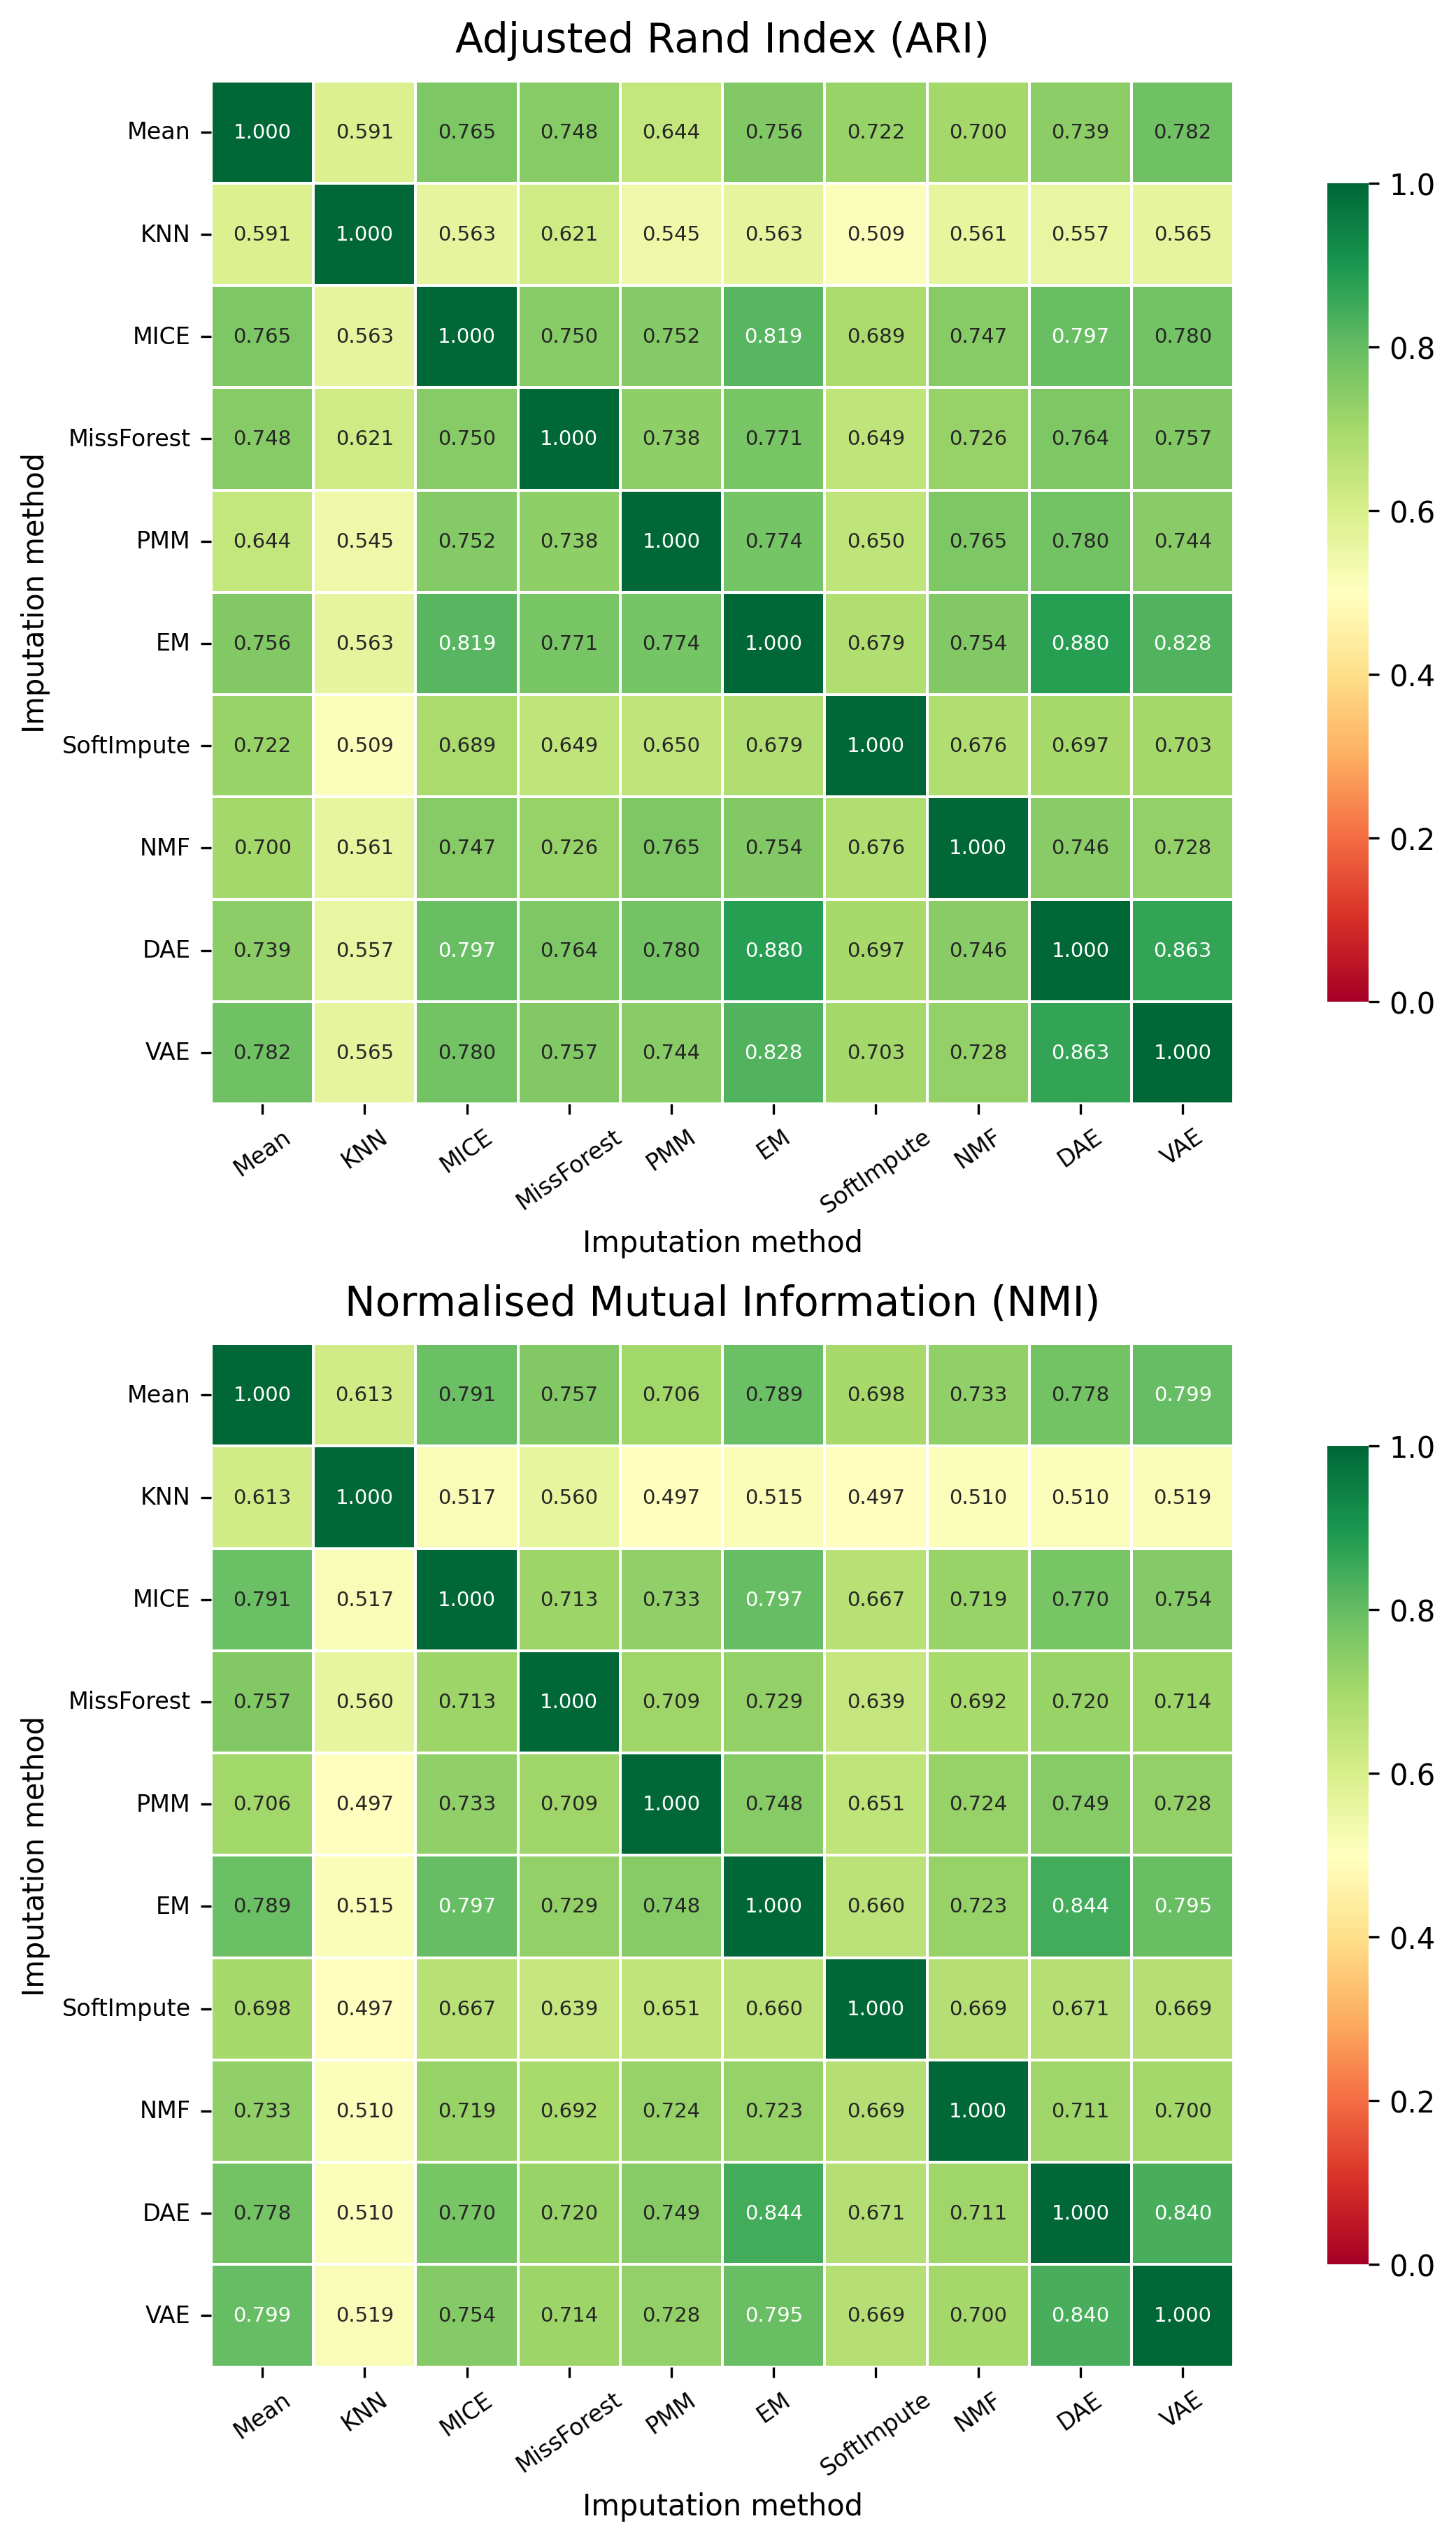
\includegraphics[width=0.88\textwidth]{Figures/h2_ari_nmi_heatmap.png}
\captionof{figure}[ARI and NMI heatmap across imputation methods]{Adjusted Rand Index (ARI) at top and normalised mutual information (NMI) at bottom for pairwise comparisons across the 10 different imputation methods. High agreement was found throughout, although KNN showed lower agreement with the smoother model-based methods.}
\label{fig:h2_ari_nmi}
\end{center}

\begin{center}
\centering
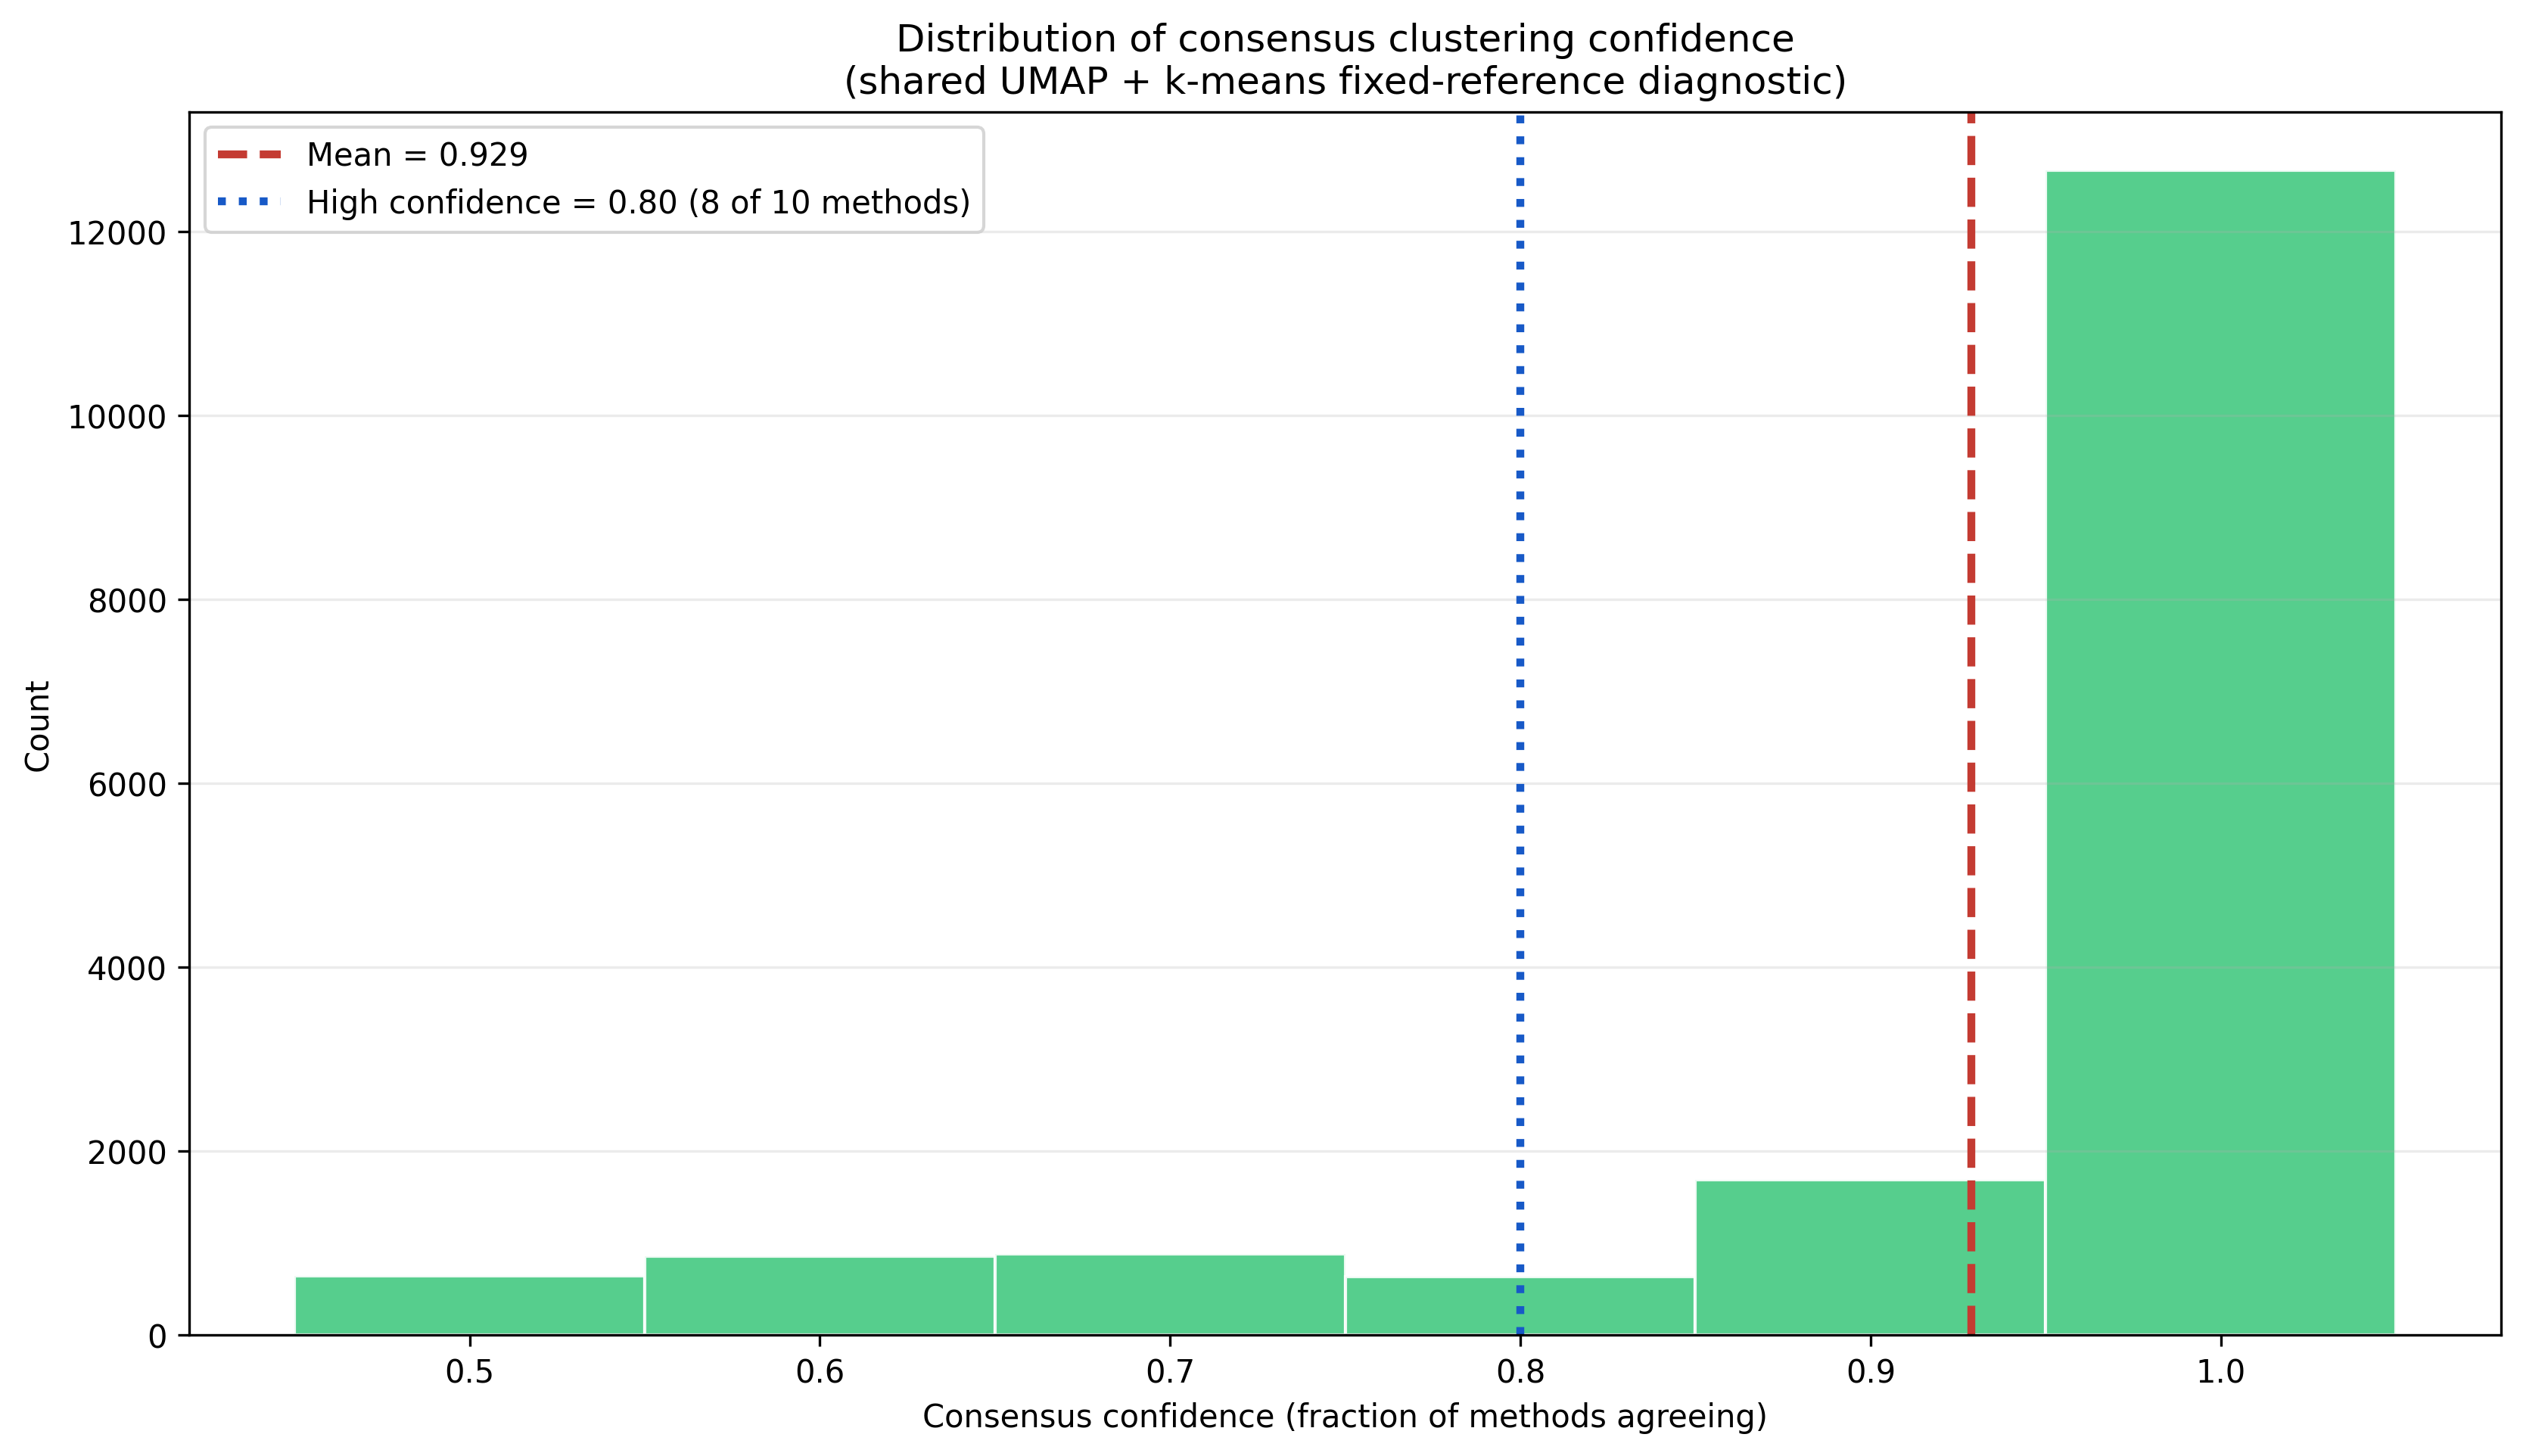
\includegraphics[width=0.85\textwidth]{Figures/h2_consensus_confidence.png}
\captionof{figure}[Consensus clustering confidence]{Histogram of consensus confidence values under the fixed-reference H2 diagnostic. The blue reference line marks the pre-defined high-confidence threshold of 0.80, equivalent to agreement by at least eight of the ten imputation methods. Mean confidence was 0.929, and 86.2\% of assessments met this threshold.}
\label{fig:h2_consensus}
\end{center}

\begin{center}
\centering
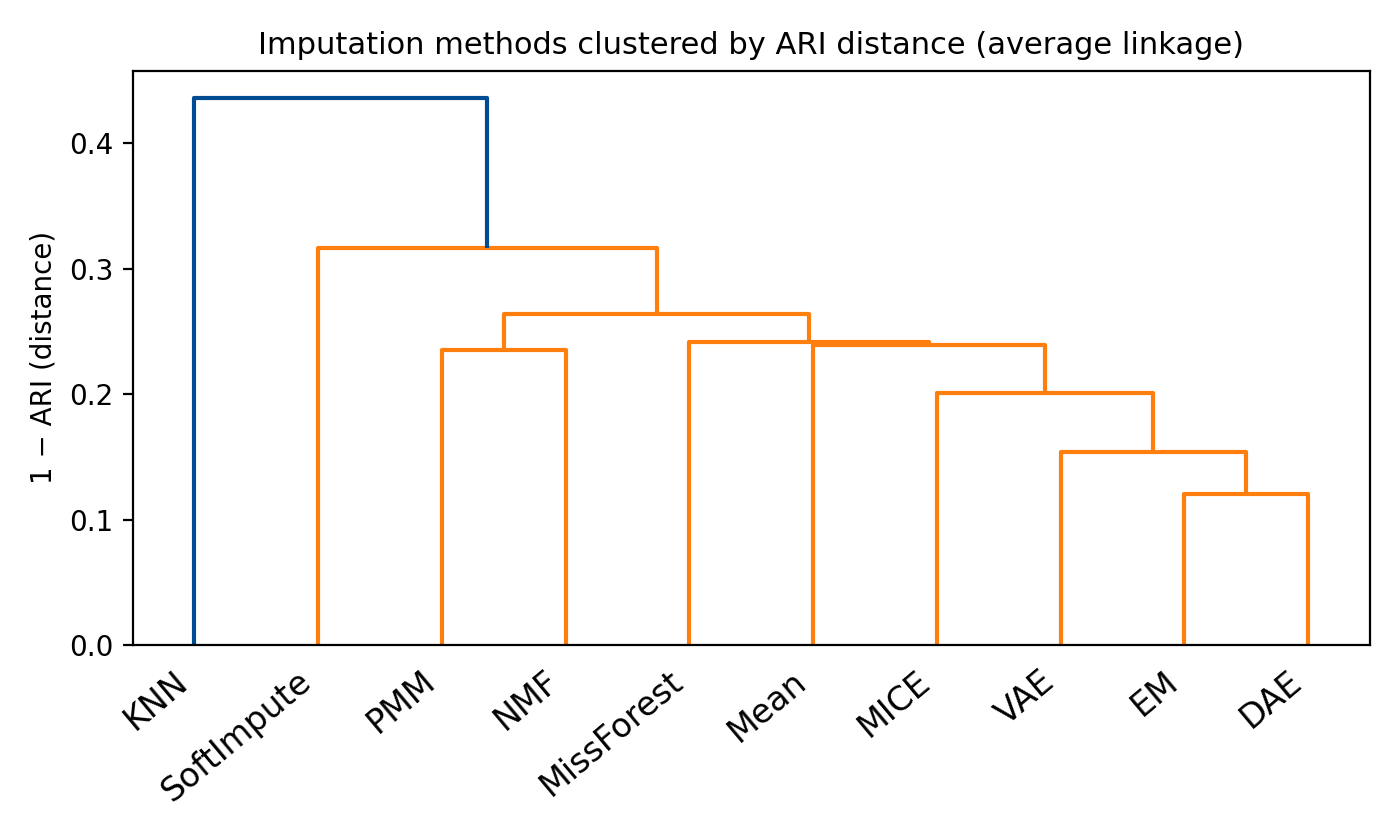
\includegraphics[width=0.85\textwidth]{Figures/h2_method_dendrogram.png}
\captionof{figure}[Method dendrogram based on ARI distance]{Dendrogram of imputation methods using average linkage clustering on ARI-based distance metrics. KNN separates itself from other branches, and tighter grouping occurs among the smoother model-based methods.}
\label{fig:h2_dendrogram}
\end{center}

\section{Hypothesis 3: Clinical Unit Association}\label{sec:h3_results}
Hypothesis 3 tests whether cognitive-severity tier is associated with clinical-unit assignment. The chi-square test showed a statistically significant association ($\chi^2 = 911.3$, $p \approx 4 \times 10^{-156}$), with Cramér's \(V=0.162\). This is a small effect by Cohen's descriptive criteria but exceeds the pre-specified threshold of 0.10. Across five independent MICE imputations, mean Cramér's \(V\) was similar at 0.154; this is an across-imputation sensitivity summary rather than a Rubin-pooled inferential estimate.

A stratified sensitivity analysis indicated that the association remained after accounting for the broad diagnostic grouping supplied by the clinical-unit lookup. Because that grouping is derived from the same lookup as detailed unit assignment, this result should not be interpreted as independent predictive validation.

The patient-grouped multinomial sensitivity analysis provided no clear evidence that tier improved out-of-sample classification of detailed clinical unit beyond the broad diagnostic grouping. Diagnosis-only log loss was 0.6064, compared with 0.6051 after adding tier (improvement 0.0013; 95\% patient-bootstrap CI $[-0.0006,0.0031]$). Accuracy was 0.7772 versus 0.7770, and macro-F1 was 0.476 versus 0.480. I therefore conclude that H3 is supported as an association hypothesis only; the present analyses do not establish added predictive value.

\begin{center}
\centering
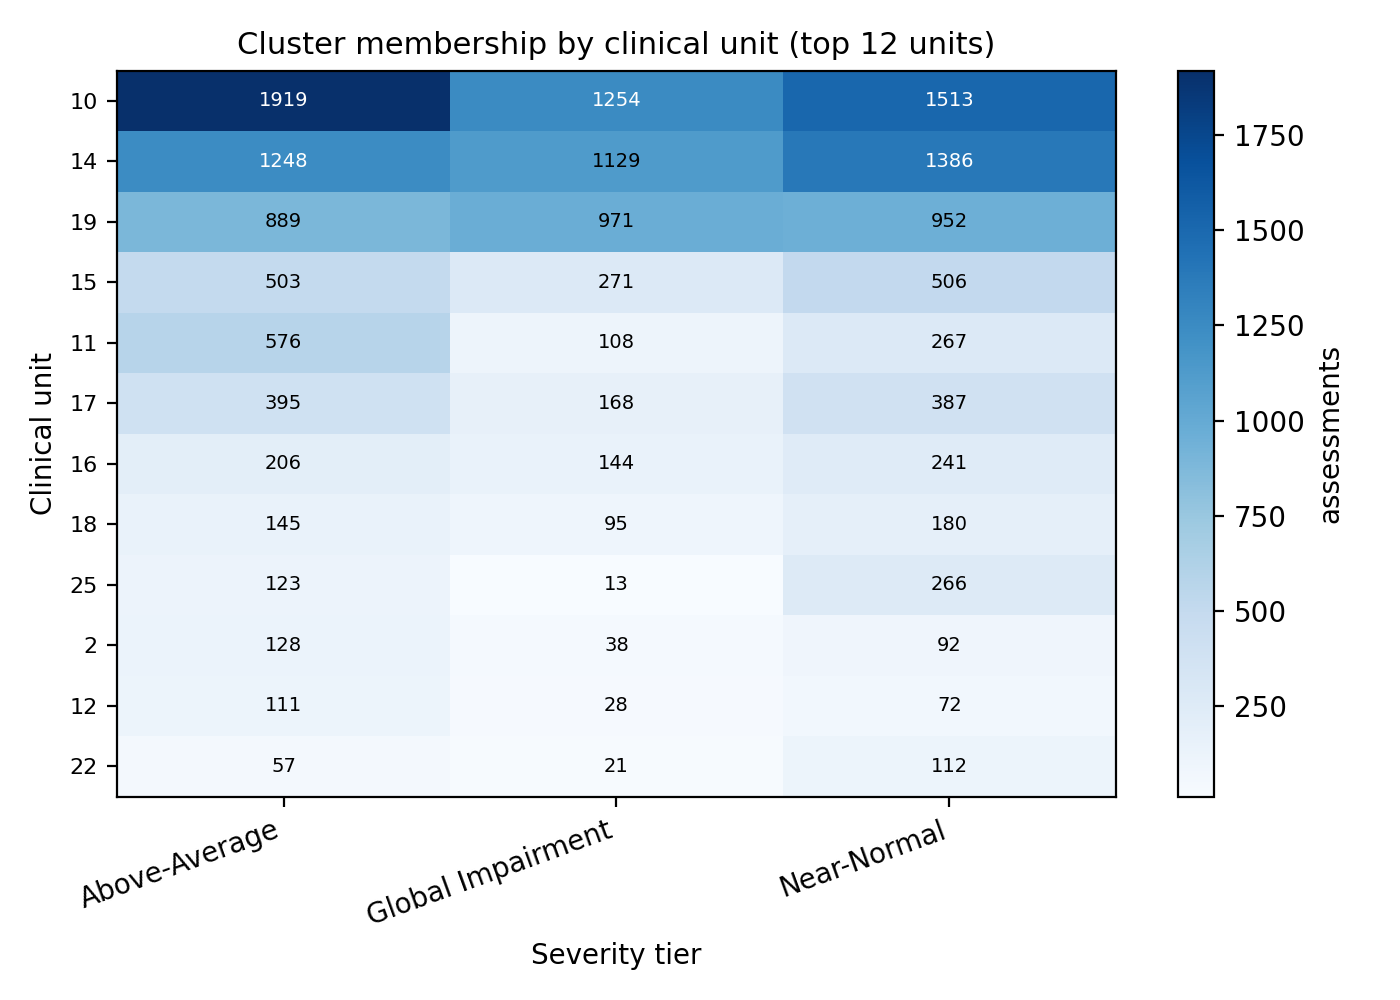
\includegraphics[width=0.9\textwidth]{Figures/h3_clinical_unit_heatmap.png}
\captionof{figure}[Clinical unit by cluster heatmap]{Heatmap of cluster assignments (columns) by clinical unit (rows). Cell colors represent frequencies. Specific tiers occur more frequently in certain units.}
\label{fig:h3_heatmap}
\end{center}

\section{Hypothesis 4: Feature Engineering}\label{sec:h4_results}
The main hypothesis was that domain-aggregate features would reduce redundancy and improve interpretability while retaining separation comparable to the individual variable-level representation. I compared the two representations using silhouette score, condition number, and variance inflation factors (VIFs).



Aggregate measures produced a marginally greater average silhouette score than did the individual variable-based measure (0.481 vs. 0.473; Figure~\ref{fig:h4_comparison}). More importantly, there was significant change in terms of how each set of measures conditioned the feature space. The average VIF decreased significantly, from 2.77 to 1.88, and the condition number decreased similarly, from 61.7 to 11.8. High VIFs indicate multicollinearity, which distorts computation of distances needed to perform the UMAP and HDBSCAN algorithms. Therefore, the decrease in VIFs indicates that the aggregation process reduced redundancy while maintaining the underlying cognitive constructs measured by the tests \parencite{lezak2012neuropsychological}.



Therefore, Hypothesis 4 is supported primarily through reduced redundancy and improved numerical conditioning and interpretability. The small silhouette difference does not indicate a meaningful increase in cluster separation.

\begin{center}
\centering
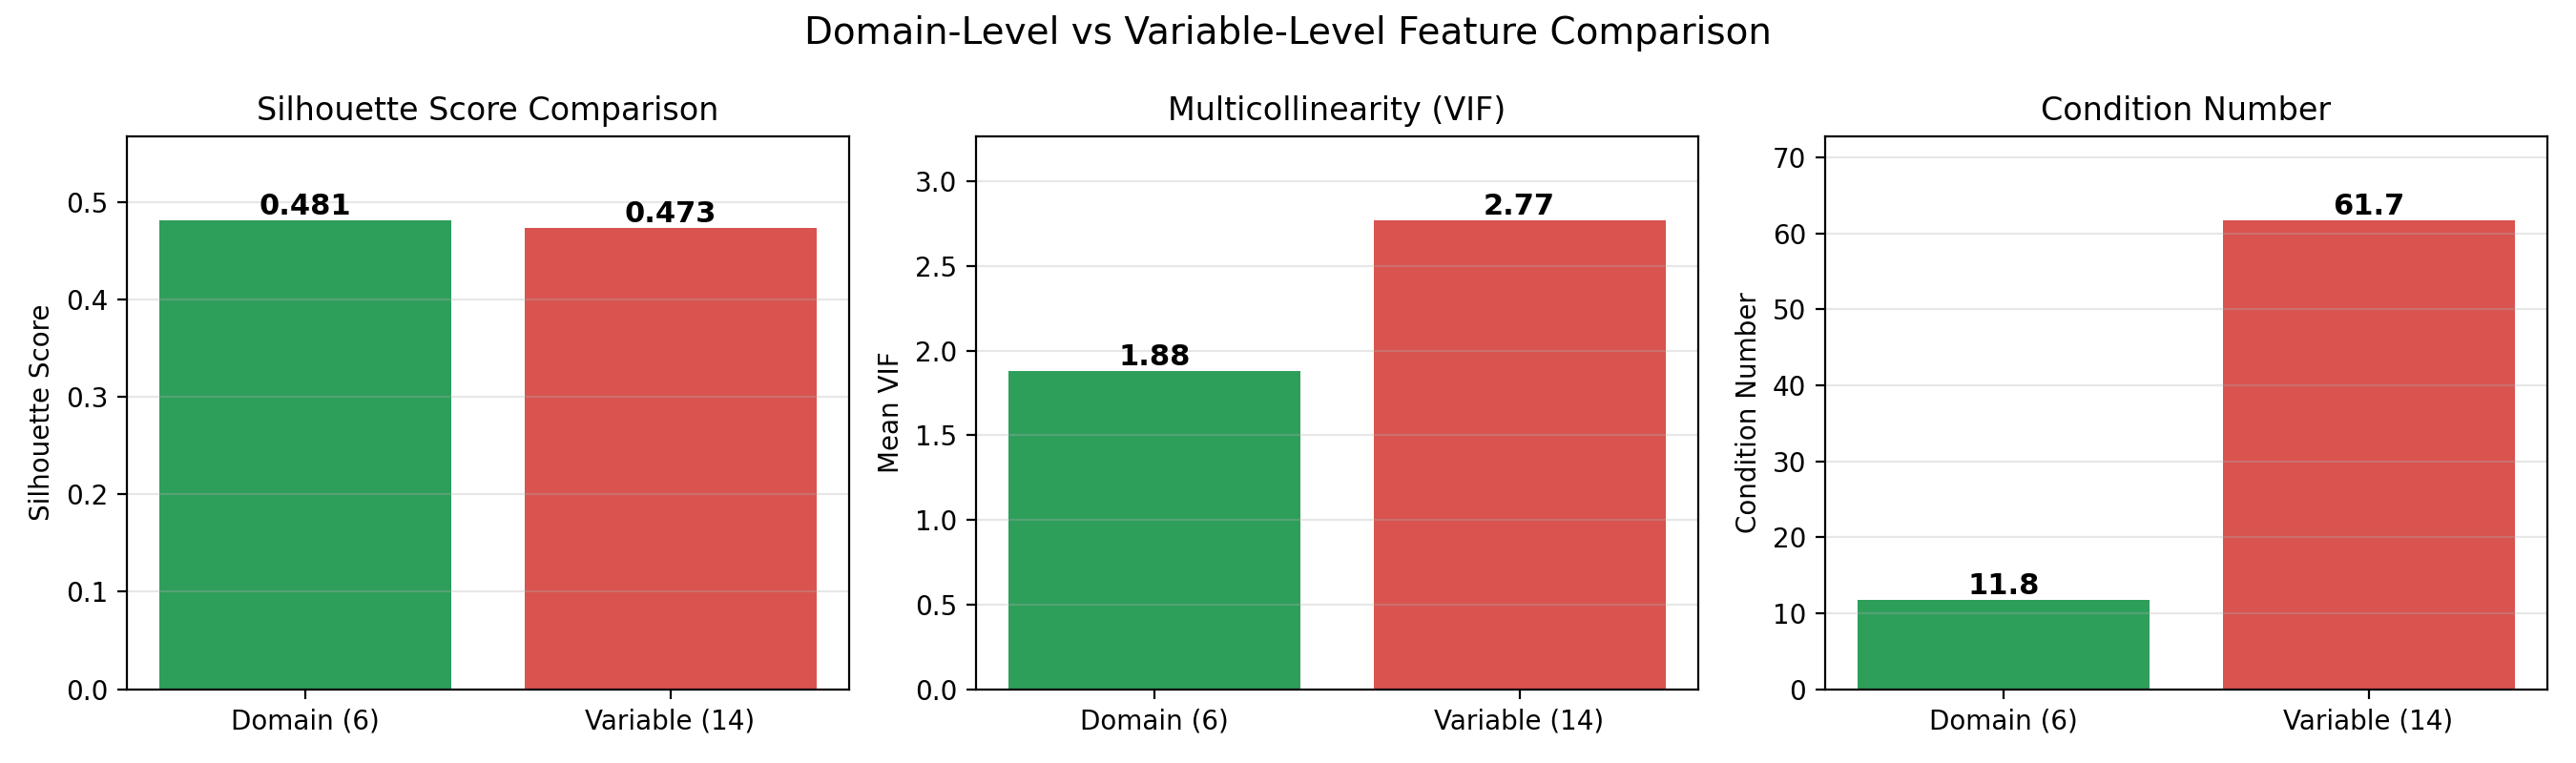
\includegraphics[width=0.95\textwidth]{Figures/h4_domain_vs_variable.png}
\captionof{figure}[Domain vs variable: silhouette, VIF, conditioning]{Comparison of domain-aggregated and variable-level features: silhouette (0.481 vs. 0.473), mean VIF (1.88 vs. 2.77), and condition number (11.8 vs. 61.7). Aggregation at the domain level produces similar separations but much less correlated, well-conditioned features.}
\label{fig:h4_comparison}
\end{center}

\section{Feature Importance Analysis}\label{sec:feature_importance}
To conduct this analysis, I trained a Random Forest surrogate model on the MICE-imputed Domain scores and used the tier labels as targets. It obtained an accuracy rate of 99.4\% in five-fold cross-validation. The accuracy of this surrogate model measures how well the tier labels can be predicted from the Domain scores. However, because the tier labels were created from the same Domain scores used in the clustering algorithm (UMAP + HDBSCAN), the surrogate model is essentially creating its own versions of the clustering boundaries. Therefore, since the surrogate model performs so well (i.e., nearly perfect accuracy), the tier labels demonstrate high degrees of separability in Domain space.



I employed Gini and permutation rankings to help illustrate the relative importance of each Domain. Orientation ranked highest (\(\text{Gini}=0.49\)), followed closely by visuoperceptual (\(\text{Gini}=0.24\)) and language (\(\text{Gini}=0.17\)), with attention (\(\text{Gini}=0.03\)) and executive function (\(\text{Gini}=0.02\)) last among the six domains (Figure~\ref{fig:feature_importance}). Although this order may provide some useful information about the importance of each Domain in terms of their relationships to one another, this ordering should be interpreted cautiously. It represents only what is internal to the clustering methodology and has been influenced partially by circularity. Additionally, Gini importance is biased when predictors are highly correlated \parencite{boulesteix2012overview}. As stated earlier, the six domains are highly positively correlated (both theoretically as part of the cognitive positive manifold and empirically as indicated by the first principal component in §\ref{sec:cluster_profiles}). Once a tree splits on a highly correlated Domain like orientation, attention appears redundant. Thus, even though attention ranks lowest, it is incorrect to infer that attention is clinically irrelevant. Rather, attention's position is best understood within the context of Figure~\ref{fig:radar_profiles} where the concentric profiles and principal component loadings determine whether the tiers represent total clinical severity or a Domain-specific dissociation.

\begin{center}
\centering
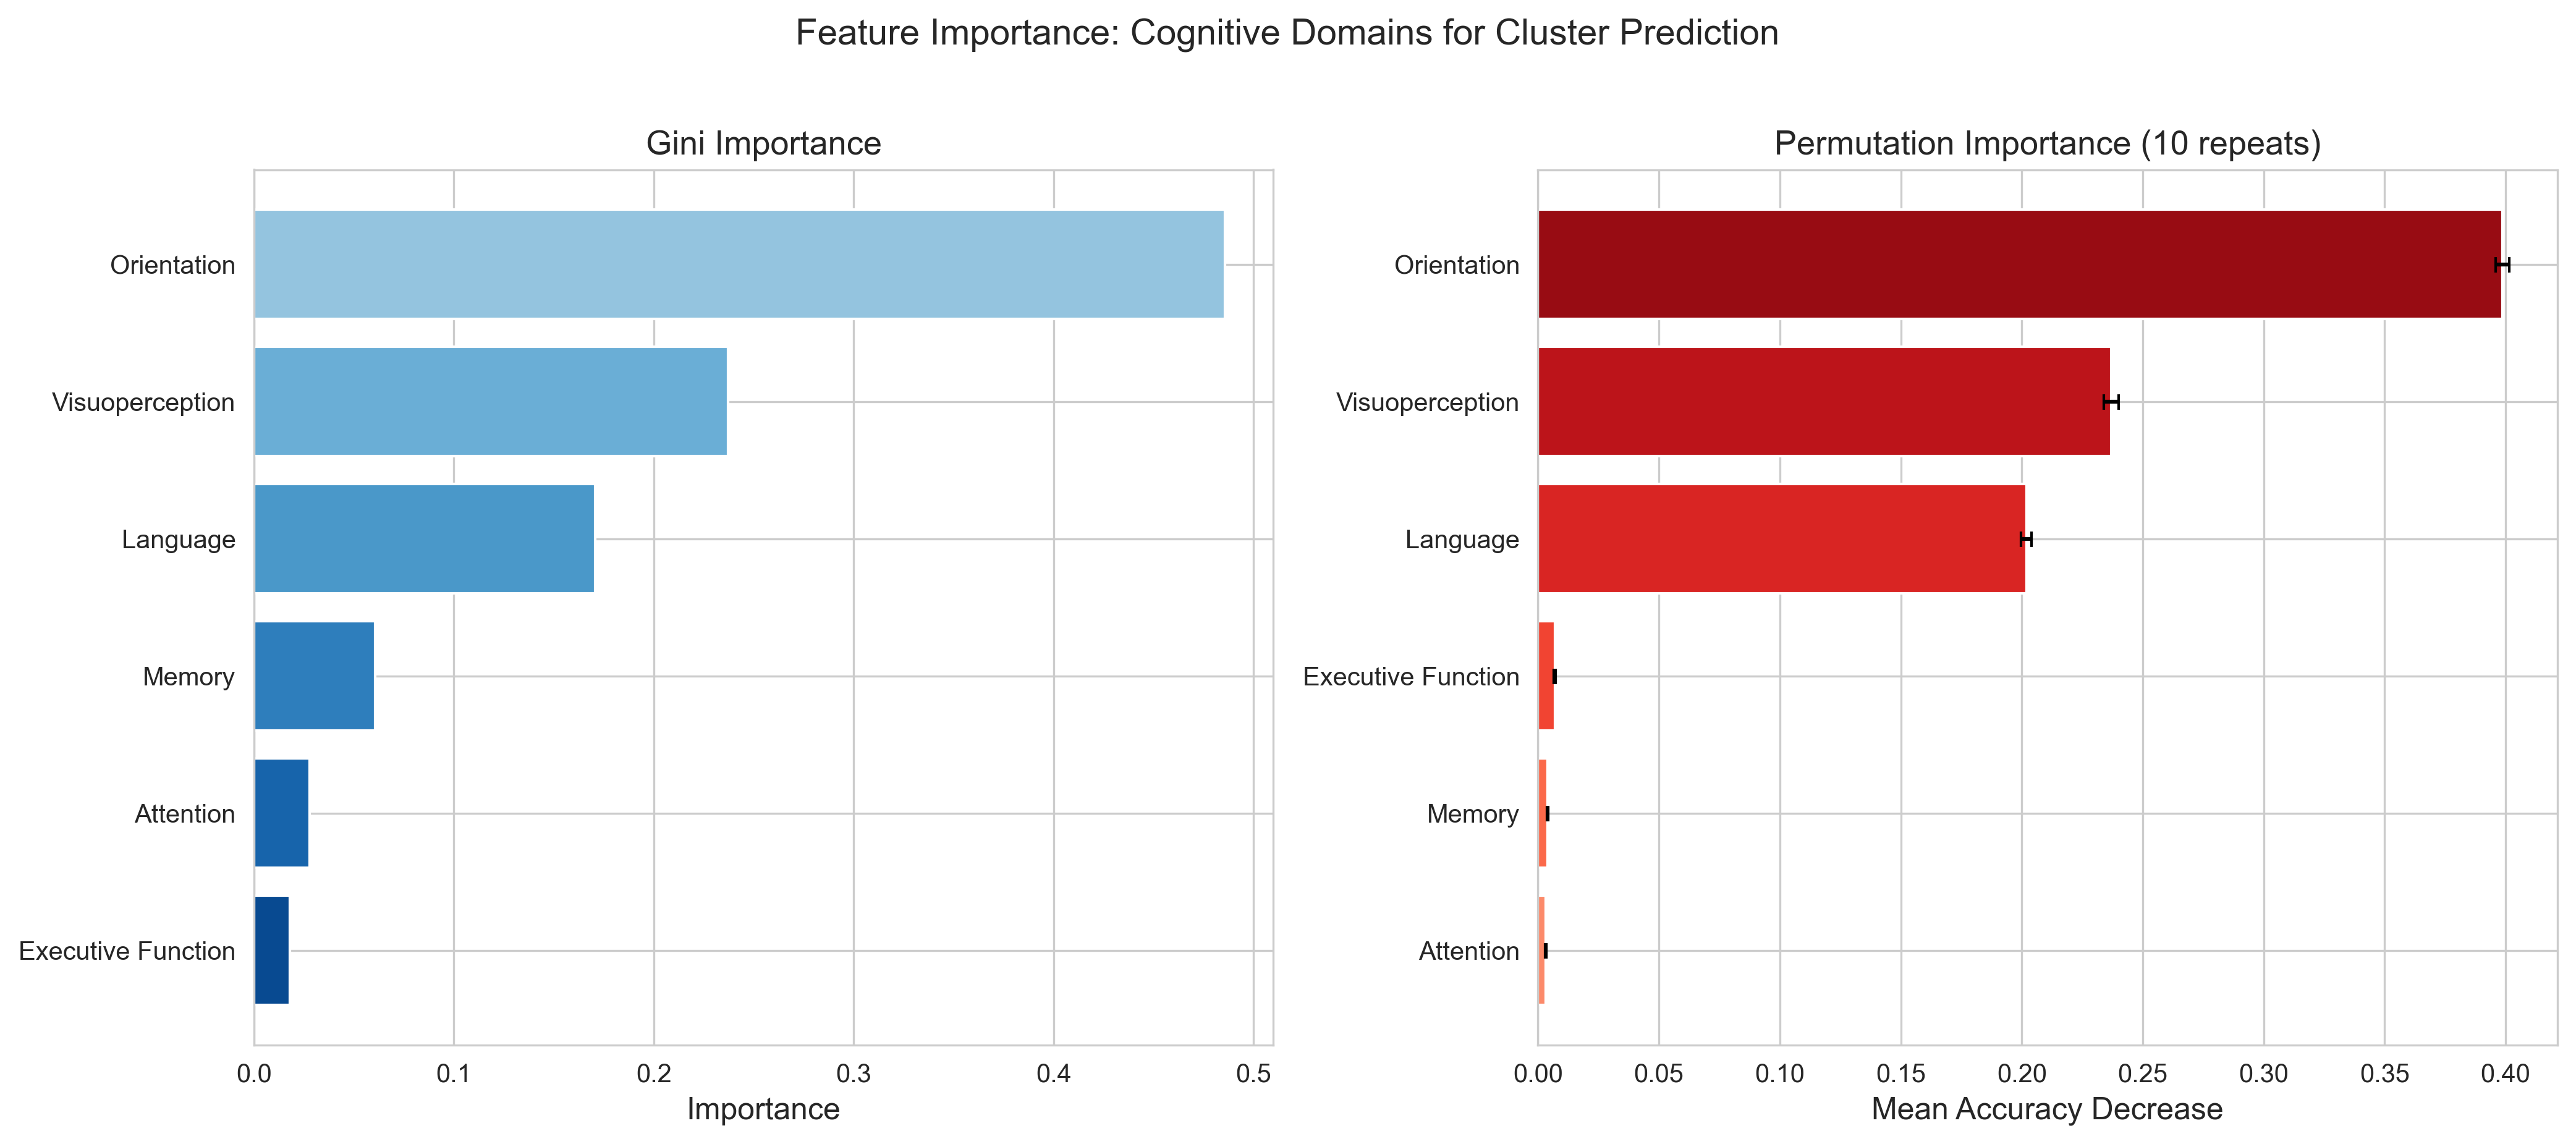
\includegraphics[width=0.9\textwidth]{Figures/feature_importance.png}
\captionof{figure}[Feature importance for cluster prediction]{Random Forest surrogate trained to recover tier labels from domain scores. Left: Gini importance. Right: Permutation importance with error bars. Since labels are derived from the same scores, this panel describes the decision boundaries of the clustering partitions rather than independently evaluating their relative importance. Because the domains are strongly intercorrelated, rankings should not be taken as implying clinical insignificance of attention.}
\label{fig:feature_importance}
\end{center}

\section{Robustness Analyses}\label{sec:robustness}
There are several analyses that help clarify the robustness of the hypotheses. First, I used a "listwise deletion" baseline. Second, I conducted a subsampling stability study. Third, I estimated bootstrap confidence intervals. Fourth, I compared results across independent MICE imputations. Fifth, I validated the findings using time since injury as an alternative measure. Finally, I used multiple comparison corrections for the 45 pairwise H2 tests.



\textbf{Bootstrap Confidence Intervals.} I performed a nonparametric bootstrap analysis at the assessment level. For the major estimates, I obtained very narrow 95\% confidence intervals around the estimated effects. For example, the bootstrap 95\% confidence interval for the H2 mean ARI is 0.710 [0.704, 0.716]; for H3, it is 0.16 [0.15, 0.18] (Cramér's V); and for H4, it is 0.05 [0.04, 0.06] (silhouette gap). These intervals reflect 17{,}406 assessment records, not 7{,}285 independent patients. Because follow-up assessments from the same patient were resampled independently, within-patient dependence was ignored; the intervals may therefore be too narrow and apparent stability may be inflated. They should not be interpreted as patient-level uncertainty estimates.



\textbf{H2 \& Multiple Comparison Correction.} In order to test H2, I needed to perform 45 different pairwise ARI comparisons against a cutoff of greater than 0.5. Therefore, I applied Holm-Bonferroni corrections to ensure family-wise Type I error rates, and Benjamini-Hochberg corrections to ensure false discovery rates. Using a parametric one-sided bootstrap p-value for each pair, under both types of corrections, the null is rejected for 44 of the 45 pairs; the only exception is KNN-SoftImpute (bootstrap mean \(\mathrm{ARI}=0.509\), 95\% CI [0.497, 0.521]). Thus, with respect to imputation robustness, all method pairs are significant except this one borderline case.



\textbf{Across-Imputation Sensitivity Summary.} I generated \(M = 5\) independent MICE imputations and ran the entire pipeline on each. For each nonlinear statistic, I report the across-imputation mean \(\bar{Q}\) and a descriptive dispersion interval calculated as \(\bar{Q} \pm t_{0.975,4}\sqrt{(1+1/M)B}\), where \(B\) is the sample variance of the five estimates. This calculation uses between-imputation variation only. Because no within-imputation variance was estimated, and because Cramér's V and silhouette are nonlinear statistics, these intervals are not interpreted as Rubin-rule confidence intervals. They are sensitivity summaries showing how results vary across plausible imputations. Mean Cramér's V was 0.154 with a descriptive interval of [0.049, 0.259], and the mean silhouette gap was 0.050 [0.043, 0.058]. The recovered number of clusters varied from 3 to 7, while domain-level features outperformed variable-level features in all five runs.



\textbf{Listwise Deletion Baseline.} If I discard the 46.9\% of the assessments with missing values and apply the pipeline only to the remaining 9{,}245 complete cases, I obtain two clusters with a silhouette of 0.257. Additionally, agreement between the MICE solution for those same patients and the solution based solely on complete cases is moderate (ARI 0.625, NMI 0.519), yet they are clearly not equivalent. Hence, imputation has a material impact upon the analysis: discarding the 46.9\% of the assessments with missing values changes both the quality and quantity of tiers recovered.



\textbf{Subsampling Stability.} When processing random 80\% subsamples of the cohort using UMAP+HDBSCAN, I find that the majority of samples recover the same general severity structure; however, exact labels and numbers of clusters vary from two to five. This is precisely what would be expected if I were converting a continuous gradient into discrete categories and is consistent with the per-cluster Jaccard results for H1.



\textbf{Missingness Threshold Sensitivity.} I also re-ran the entire process -- including variable selection; domain computation; MICE imputation; and UMAP+HDBSCAN -- at five Tier 1 thresholds from 30\% to 70\%. As shown in Figure~\ref{fig:sensitivity}, the solution remains in the two to three tier range with silhouettes ranging from 0.39 to 0.52 over thresholds of 40\% to 70\%. Only at 30\%, where the analysis becomes overly restrictive with regards to how many variables are allowed, does the solution break down. Therefore, the 50\% threshold used throughout the main analysis represents a reasonable balance between how much information is present in each record and how many variables are available.

\begin{center}
\centering
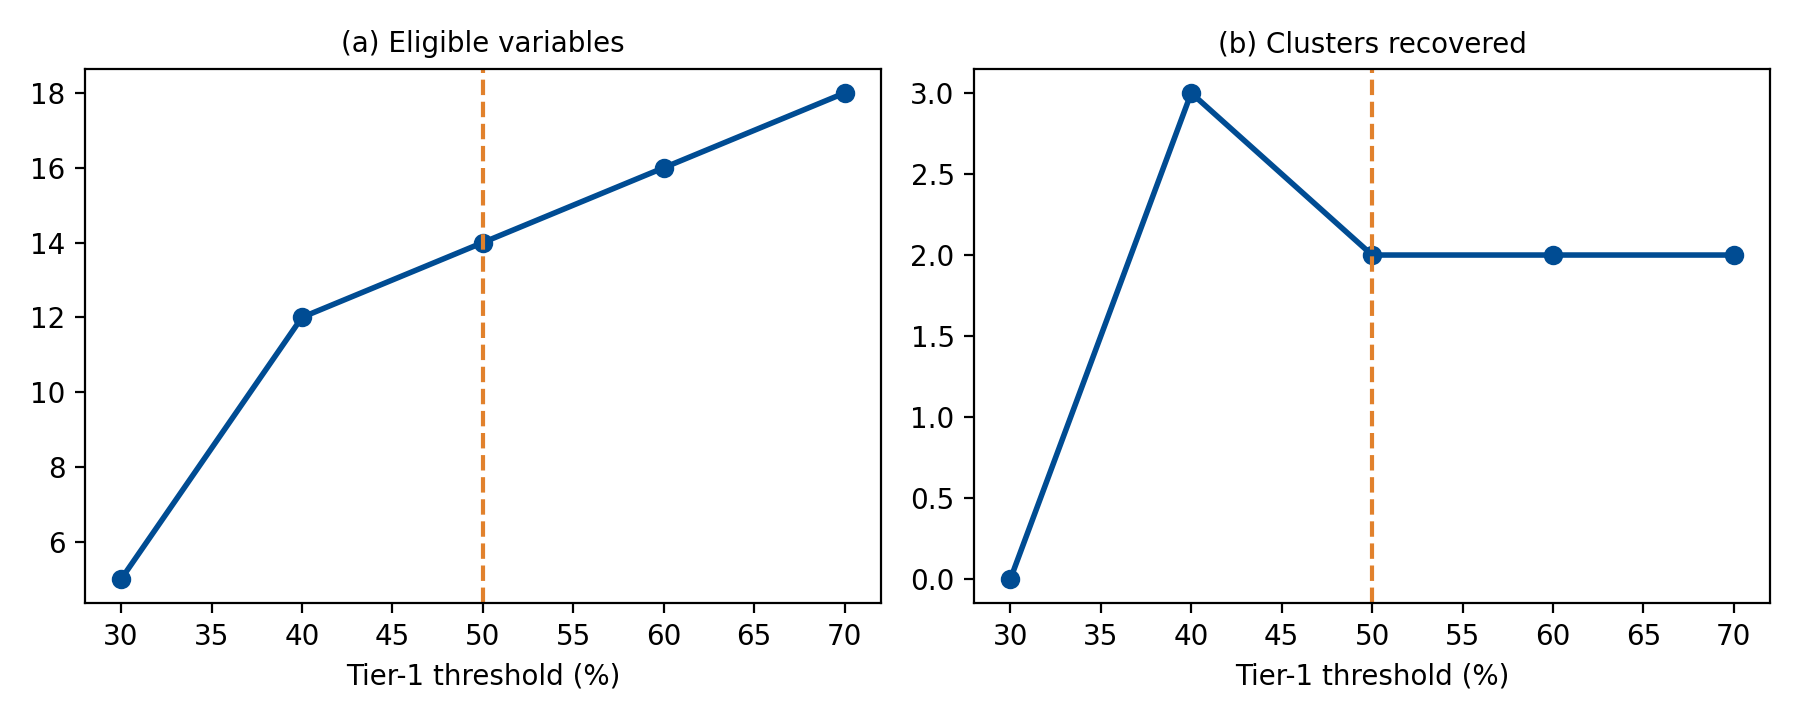
\includegraphics[width=0.8\textwidth]{Figures/sensitivity_analysis_a.png}\\[0.5em]
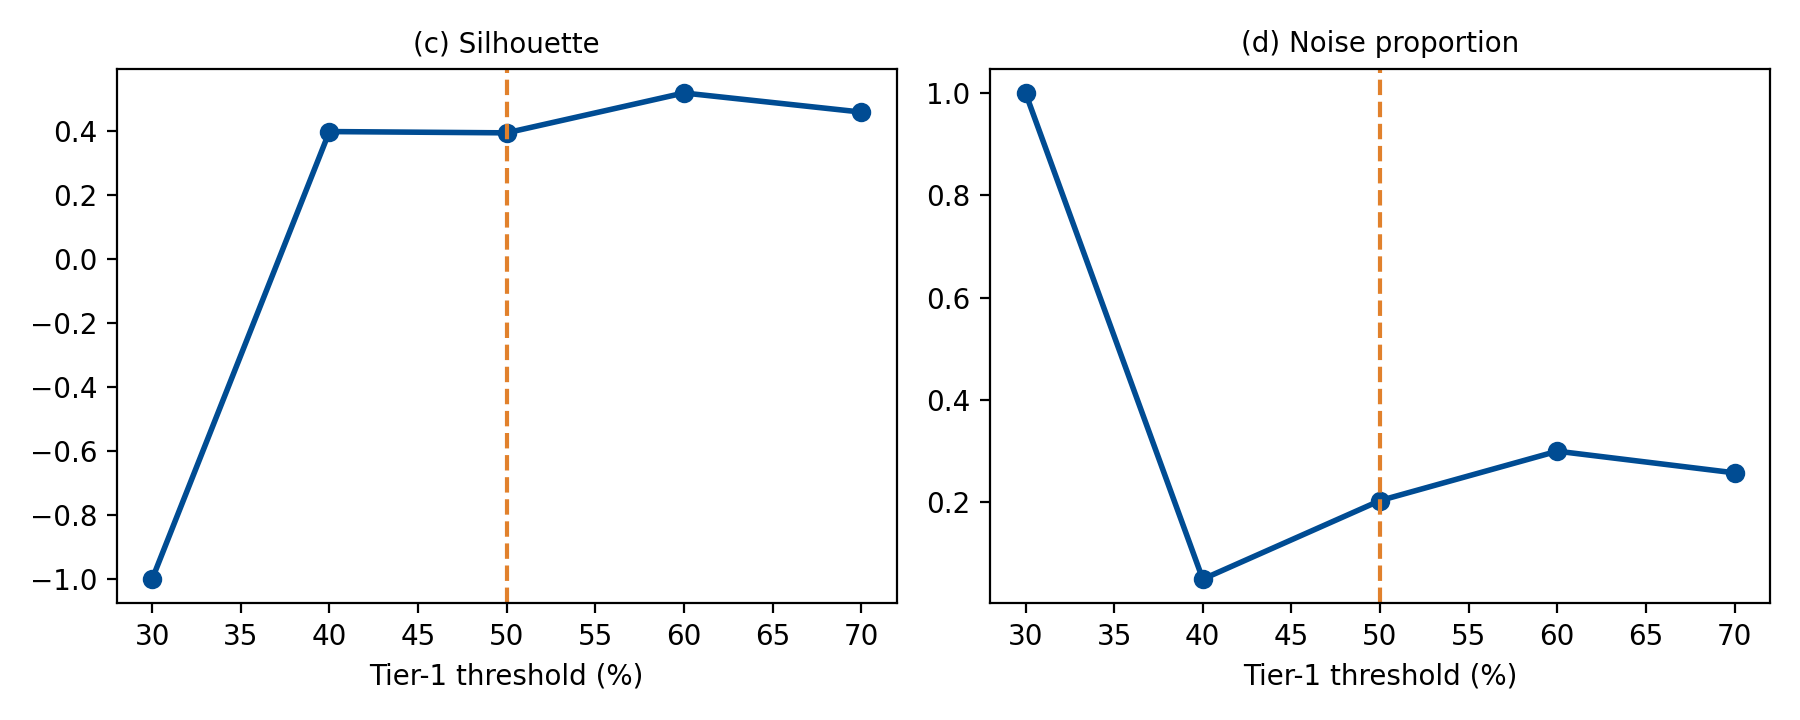
\includegraphics[width=0.8\textwidth]{Figures/sensitivity_analysis_b.png}
\captionof{figure}[Sensitivity to missingness threshold]{Effect of varying Tier~1 missingness threshold across five values (30 -- 70\%). Upper row: (a) Number of available variables and (b) Number of clusters identified. Lower row: (c) Silhouette score and (d) Proportion of noise. Vertical dashed lines indicate Tier~1 missingness threshold used in primary analyses.}
\label{fig:sensitivity}
\end{center}

\textbf{Outcome-Adjacent Validation.} Although functional outcomes are unavailable for use as validating measures of impairment status at discharge, I examined functional change through time-since-injury (TSI) at each assessment as an alternate validating measure. TSI varies significantly by tier (Kruskal-Wallis test $p = 4 \times 10^{-28}$), with median TSI times of 214 days for Above Average, 188 days for Near Normal, and 172 days for Global Impairment. Thus, as TSI increases, severity of impairment decreases across these three tiers. Among the 5{,}206 patients who have had at least two assessments, 50.2\% (2{,}613 patients) maintain their original tier assignment while 49.8\% (2{,}593 patients) experience some degree of tier shift. While such movement could suggest that patients possess a set of fixed phenotypic characteristics, such movement is far more indicative of variability in severity along a spectrum of impairment severity. Furthermore, among the 912 patients who experienced exactly two assessments and changed tiers during that period, improvement in functional status occurred approximately three times as frequently as worsening in functional status (706 vs. 206 transitions), consistent with expectations regarding natural clinical recovery patterns.



\textbf{Embedding Seed Stability.} To determine whether the clustering was due to UMAP's random initialization, I repeated the entire embedding and clustering process on the MICE-imputed domain scores using ten randomly selected seeds with equal hyperparameter settings. There was high concordance between labeling schemes; specifically, the mean pairwise ARI across the ten runs was 0.957 (median \(= 0.960\), min-max \(= [0.900, 1.000]\)). After k-nearest neighbor reassignment, this increased to 0.965. With respect to my finding that there exists a strong underlying severity axis supported by deterministic PCA (see §\ref{sec:cluster_profiles}), together with embedding seed stability, this further decreases concerns that the solution was simply an artifact of unstable UMAP initialization.



\textbf{Gaussian Mixture / Latent Profile Baseline.} As a model-based comparison, I fit Gaussian mixture models with full covariance matrices to the imputed domain scores for \(k\) varying from 2 through 6. This analysis is analogous to latent profile analysis in that it estimates model-based continuous-profile classes, but it is not a formal latent profile analysis with full-information maximum likelihood on the incomplete raw data. BIC decreased monotonically with \(k\) (from 243{,}249 at \(k = 2\) to 92{,}606 at \(k = 6\)). This shows only that no BIC optimum was reached within the tested range; it does not establish a continuum, and a solution with more than six components might have been preferred. Mixture-model solutions agreed only modestly with the density-based tiers (\(\mathrm{ARI} = 0.350-0.400\)), while the two-component solution had the clearest silhouette (0.45). I therefore treat this baseline as inconclusive about class number. The continuum interpretation rests primarily on the concentric domain profiles, the dominant first principal component, weak original-space silhouette, and sensitivity of tier count. A formal latent profile analysis with FIML and a wider class range remains a separate model-based extension.



\textbf{MNAR Tipping Point.} To establish bounds on potential missing-not-at-random mechanisms, I assumed every missing value was replaced by the worst observed performance on that variable -- either the minimum value or the maximum value depending on whether it was a timed ATMTA or not. Clearly, this is an intentionally extreme and conservative assumption. Under this condition, even though the partition became fractured and the silhouette fell to 0.030 because point-mass spikes were created when all missing values were forced to extreme values, a distinct lowest severity tier still existed and retained approximately 65.2\% of assessments originally labeled as Global Impairment. Therefore, even under extreme MNAR assumptions, Global Impairment is likely the most robust portion of the solution. Most importantly, extreme MNAR assumptions seem to degrade finer separation within lower severity tiers, and thus a formal delta-shifted tipping-point analysis seems like an interesting future direction.



\textbf{Summary Characteristics of Excluded Records.} Applying the Tier-1 filter to the full raw cohort retained 17{,}406 of the 22{,}075 records used in the source extract and excluded 4{,}669 records. Discarded records averaged only 0.800 of their 14 eligible tests, whereas retained records averaged 12.5 tests per record, thereby appearing to represent nearly empty administrative encounters instead of incomplete testing of severely impaired individuals. Demographically, both excluded records and retained records are largely indistinguishable (e.g., age at injury: 45.7 vs. 46.3 years; Cohen's \(d = -0.04\); sex: male/female = [63\%;37\%] vs. [68\%;32\%]; TSI: 2.3 vs. 1.6 years; \(d = 0.16\)). Therefore, I do not believe that the Tier-1 filter suppresses detection of a cognitively impaired subgroup identifiable via measurable characteristics -- although I cannot assess cognitive impairment directly in the excluded records.

\section{Cluster Clinical Naming}\label{sec:cluster_names}
To give the density-based clusters clinically relevant labels, I employed a rule-based naming system based upon the domain-level z-score profiles associated with each cluster.



Clustering profiles associated with domains having z-scores greater than +0.5 were labeled Above Average.



Profiles associated with domains having z-scores less than -0.5 were labeled Global Impairment.



All other profiles were labeled Near Normal.



This resulted in the final labels being Above Average ($n = 6{,}725$), Near Normal ($n = 6{,}328$), and Global Impairment ($n = 4{,}353$).



Since the tiers differ primarily in terms of overall level and not profile shape -- severity labels are preferable to phenotype names.



They provide valuable shorthand for clinicians engaged in discussing potential rehabilitation options with their patients -- as well as providing useful tier-based guidance for rehabilitation triaging efforts.



The full mapping of identifier codes to assessment frequency is contained within the interactive CogDash dashboard
